\documentclass[a4paper,12pt]{article}
\usepackage[utf8]{inputenc}
\usepackage[T1]{fontenc}
\usepackage[italian]{babel}
\usepackage[sfdefault]{atkinson}
\renewcommand*\familydefault{\sfdefault}
\usepackage{float}
\usepackage{microtype}
\usepackage{geometry}
\usepackage{setspace}
\usepackage{enumitem}
\usepackage{titlesec}
\usepackage{chngpage}
\usepackage{pdflscape}
\usepackage{tocloft}
\usepackage{longtable}
\usepackage{ltablex}
\usepackage{array}
\usepackage{graphicx}
\usepackage{fancyhdr}
\usepackage[table]{xcolor}
\usepackage{color,soul}
\usepackage[most]{tcolorbox}
\usepackage{nameref}
\usepackage[colorlinks=true]{hyperref}
\usepackage{tabularx}
\usepackage{adjustbox}
% Colori ZPUS - Verde, Nero, Bianco
\definecolor{zpusgreen}{RGB}{4, 138, 55}
\definecolor{zpusdarkgreen}{RGB}{0, 100, 0}
\definecolor{zpusblack}{RGB}{0, 0, 0}
\definecolor{zpuswhite}{RGB}{255, 255, 255}
\definecolor{zpuslightgray}{RGB}{245, 245, 245}
\definecolor{codewordcolor}{RGB}{49, 127, 69}


\usepackage{tikz}
\usepackage{pgfplots}
\pgfplotsset{compat=1.17}

\hypersetup{
    linkcolor=black,
    urlcolor=blue
}

\definecolor{lightblack}{gray}{0.35}
\newcommand{\glossario}[1]{\textit{#1}\textsubscript{\textbf{\textit{\textcolor{lightblack}{G}}}}}
\newcommand{\ped}[1]{\textsubscript{#1}}
\newcommand{\codeword}[1]{{\textcolor{codewordcolor}{\textit{\text{#1}}}}}
\renewcommand{\tabularxcolumn}[1]{m{#1}}
\newcolumntype{Y}{>{\raggedright\arraybackslash}X}
\def\UrlBreaks{\do\_\do\,\do\:\do\-\do\.\do\/}

\pagestyle{fancy}
\setlength{\headwidth}{\textwidth}
\fancyhfoffset[L,R]{0pt}
\lhead{\rightmark}
\rhead{7-ZPUs}
\lfoot{Specifica Tecnica}
\rfoot{\thepage}
\cfoot{}
\renewcommand{\headrulewidth}{0.8pt}
\renewcommand{\footrulewidth}{0.8pt}

\renewcommand{\contentsname}{Indice}
\renewcommand{\listoftables}{Elenco delle tabelle}
\renewcommand{\listoffigures}{Elenco delle immagini}

\geometry{margin=2.5cm}
\setstretch{1.1}

\titleclass{\subsubsubsection}{straight}[\subsection]

\newcounter{subsubsubsection}[subsubsection]
\renewcommand\thesubsubsubsection{\thesubsubsection.\arabic{subsubsubsection}}
\renewcommand\theparagraph{\thesubsubsubsection.\arabic{paragraph}} % optional; useful if paragraphs are to be numbered

\titleformat{\subsubsubsection}
  {\normalfont\normalsize\bfseries}{\thesubsubsubsection}{1em}{}
\titlespacing*{\subsubsubsection}
{0pt}{3.25ex plus 1ex minus .2ex}{1.5ex plus .2ex}

\makeatletter
\renewcommand\paragraph{\@startsection{paragraph}{5}{\z@}%
  {3.25ex \@plus1ex \@minus.2ex}%
  {-1em}%
  {\normalfont\normalsize\bfseries}}
\renewcommand\subparagraph{\@startsection{subparagraph}{6}{\parindent}%
  {3.25ex \@plus1ex \@minus .2ex}%
  {-1em}%
  {\normalfont\normalsize\bfseries}}
\def\toclevel@subsubsubsection{4}
\def\toclevel@paragraph{5}
%\def\toclevel@paragraph{6}
\def\toclevel@subparagraph{6}
\def\l@subsubsubsection{\@dottedtocline{4}{7em}{4em}}
\def\l@paragraph{\@dottedtocline{5}{10em}{5em}}
\def\l@subparagraph{\@dottedtocline{6}{14em}{6em}}
\makeatother

\setcounter{secnumdepth}{4}
\setcounter{tocdepth}{4}

\titleformat{\section}{\LARGE\bfseries}{\thesection}{1em}{}
\titleformat{\subsection}{\Large\bfseries}{\thesubsection}{1em}{}
\titleformat{\subsubsection}{\large\bfseries}{\thesubsubsection}{1em}{}
\titleformat{\paragraph}{\large\bfseries}{\theparagraph}{1em}{}
\titleformat{\subparagraph}{\normalsize\bfseries}{\thesubparagraph}{1em}{}

\setlength\parindent{0pt}


\begin{document}

\pagenumbering{roman}

\pagenumbering{arabic}
\setcounter{page}{1}


\begin{center}
    \includegraphics[width=9.5cm]{../../assets/logo7ZPUs.jpg}\\
    \small\hspace{10cm} 7zpus.swe@gmail.com\\
    \vspace{0.5cm}
    \LARGE \textbf{Specifica Tecnica}\\
    \vspace{0.3cm}
\end{center}

\vspace{0.3cm}
\hrule
\vspace{0.5cm}


\section*{Tabella di Versionamento}
\begin{table}[H]
    \begin{adjustwidth}{-4cm}{-4cm}
    \centering
    \begin{tabular}{|c|c|c|c|c|}
        \hline
        \textbf{Versione} & \textbf{Data} & \textbf{Autore}  & \textbf{Verificatore} & \textbf{Descrizione} \\
        \hline
        0.2.0 & 2026/04/08 & Georgescu Diana & Soligo Lorenzo & Aggiunta descrizione modulo Export \\
        \hline
        0.1.0 & 2026/02/28 & Laoud Zakaria & Georgescu Diana & \begin{tabular}[c]{@{}c@{}} Creazione del documento\\ e stesura struttura iniziale \end{tabular} \\
        \hline
    \end{tabular}
    \end{adjustwidth}
\end{table}

\newpage
\tableofcontents

\newpage
\listoffigures

\listoftables

\newpage
\section{Introduzione}

\subsection{Obiettivo del documento}
L’obiettivo del presente documento è descrivere in modo rigoroso le scelte tecnologiche e l’architettura del prodotto \textit{DIPReader}, adottando il modello di progettazione \textit{C4}.\\
L’analisi verrà condotta partendo dalla descrizione del contesto applicativo, per poi approfondire la struttura dei container, delle componenti e, infine, del codice, al fine di fornire una rappresentazione completa, 
coerente e sistematica del sistema.

\subsection{Glossario}
Ogni termine tecnico o con un significato particolare nell’ambito dell’Ingegneria del Software, utilizzato nella documentazione di progetto, è definito nell’apposito documento
\href{https://7-zpus.github.io/Docs/assets/3_PB/DocumentiInterni/Glossario.pdf}{Glossario }\ped{(v2.0.0)}.

\subsection{Riferimenti}

    \subsubsection{Riferimenti normativi}
    \begin{itemize}
        \item \href{https://github.com/7-ZPUs/Docs/blob/main/3_PB/DocumentiInterni/NormeDiProgetto.pdf}{Norme di Progetto v2.0.0 }\ped{(v2.0.0)}
        \item \href{https://en.wikipedia.org/wiki/Software_design_description}{Standard SDD/IEEE/1016:2009}\ped{(ultimo accesso: 02/03/2026)}
        \item \href{https://www.math.unipd.it/~tullio/IS-1/2025/Dispense/PD1.pdf}{Regolamento di Progetto Didattico a.a.
            2025/2026} \ped{(ultimo accesso: 02/03/2026)}
    \end{itemize}

    \subsubsection{Riferimenti informativi}
    \begin{itemize}
        \item \href{https://www.math.unipd.it/~tullio/IS-1/2025/Progetto/C3.pdf}{Capitolato C3: DIPReader} \ped{(ultimo accesso: 10/02/2026)}
        \item \href{https://www.math.unipd.it/~rcardin/swea/2022/Design%20Pattern%20Architetturali%20-%20Dependency%20Injection.pdf}
        {Dispense su Dependency Injection }\ped{(Ultimo accesso: 02/03/2026)}
        \item \href{https://www.math.unipd.it/~rcardin/swea/2023/Object-Oriented%20Progamming%20Principles%20Revised.pdf}
        {Dispense su OOP }\ped{(Ultimo accesso: 02/03/2026)}
        \item \href{https://www.math.unipd.it/~rcardin/swea/2023/Diagrammi%20delle%20Classi.pdf}
        {Dispense su Diagrammi delle classi }\ped{(Ultimo accesso: 02/03/2026)}
        \item \href{https://www.math.unipd.it/~rcardin/swea/2022/Software%20Architecture%20Patterns.pdf}
        {Dispense su Pattern architetturali }\ped{(Ultimo accesso: 02/03/2026)}
        \item \href{https://www.math.unipd.it/~rcardin/swea/2022/Design%20Pattern%20Creazionali.pdf}
        {Dispense su Pattern creazionali }\ped{(Ultimo accesso: 02/03/2026)}
        \item \href{https://www.math.unipd.it/~rcardin/swea/2022/Design%20Pattern%20Strutturali.pdf}
        {Dispense su Pattern strutturali }\ped{(Ultimo accesso: 02/03/2026)}
        \item \href{https://www.math.unipd.it/~rcardin/swea/2021/SOLID%20Principles%20of%20Object-Oriented%20Design_4x4.pdf}
        {Dispense su Principi SOLID }\ped{(Ultimo accesso: 02/03/2026)}
        \item \href{https://www.math.unipd.it/~tullio/IS-1/2023/Dispense/T6.pdf}
        {Dispense sulla Progettazione software }\ped{(Ultimo accesso: 02/03/2026)}
        \item \href{https://www.math.unipd.it/~tullio/IS-1/2023/Dispense/T7.pdf}
        {Dispense sulla Qualità del software }\ped{(Ultimo accesso: 02/03/2026)}
        \item \href{https://github.com/rcardin/hexagonal}
        {Repository Architettura esagonale (Kotlin) }\ped{(Ultimo accesso: 02/03/2026)}
        \item \href{https://github.com/rcardin/hexagonal-java/}
        {Repository Architettura esagonale (Java) }\ped{(Ultimo accesso: 02/03/2026)}
        \item \href{https://github.com/rcardin/swe-imdb}
        {Repository Ingegneria del software - swe-imdb }\ped{(Ultimo accesso: 02/03/2026)}
        \item \href{https://c4model.com/}
        {C4 Model }\ped{(Ultimo accesso: 03/03/2026)}
        \item \href{https://plantuml.com/}
        {PlantUML }\ped{(Ultimo accesso: 03/03/2026)}
        \item Riferimenti a scelte tecnologiche:
        \begin{itemize}
            \item \href{https://www.typescriptlang.org/}
            {TypeScript }\ped{(Ultimo accesso: 03/03/2026)}
            \item \href{https://angular.io/}
            {Angular }\ped{(Ultimo accesso: 03/03/2026)}
            \item \href{https://www.electronjs.org/}
            {Electron }\ped{(Ultimo accesso: 03/03/2026)}
            \item \href{https://www.sqlite.org/}
            {SQLite }\ped{(Ultimo accesso: 03/03/2026)}
            \item \href{https://github.com/asg017/sqlite-vss}
            {sqlite-vss }\ped{(Ultimo accesso: 03/03/2026)}
            \item \href{https://onnxruntime.ai/}
            {ONNX Runtime }\ped{(Ultimo accesso: 03/03/2026)}
            \item \href{https://huggingface.co/docs/transformers.js}
            {Transformers.js }\ped{(Ultimo accesso: 03/03/2026)}
            \item \href{https://nodejs.org/}
            {Node.js }\ped{(Ultimo accesso: 03/03/2026)}
        \end{itemize}
        \item \href{https://7-zpus.github.io/Docs/assets/3_PB/DocumentiInterni/Glossario.pdf}{Glossario }\ped{(v2.0.0)}
        \item \href{https://github.com/7-ZPUs/Docs/blob/main/3_PB/DocumentiEsterni/PianoDiProgetto.pdf}{Piano di Progetto }\ped{(v2.0.0)}
        \item \href{https://github.com/7-ZPUs/Docs/blob/main/3_PB/DocumentiEsterni/PianoDiQualifica.pdf}{Piano di Qualifica }\ped{(v2.0.0)}
        \item Verbali interni:
        \item Verbali esterni:
    \end{itemize}
    
    

\newpage
\section{Tecnologie utilizzate}
\newpage
\section{Contesto del sistema}

\subsection{Modello architetturale}

\subsection{Descrizione degli attori esterni}

\subsection{Descrizione dei sistemi esterni}

\newpage
\section{Architettura dei container}
La progettazione del sistema \textit{DIPReader} è stata guidata dai principi di modularità, scalabilità e manutenibilità, con l'obiettivo di creare un'architettura che possa evolversi nel tempo e adattarsi a nuove esigenze e normative AGID.\\
\begin{figure}[H]
    \centering
    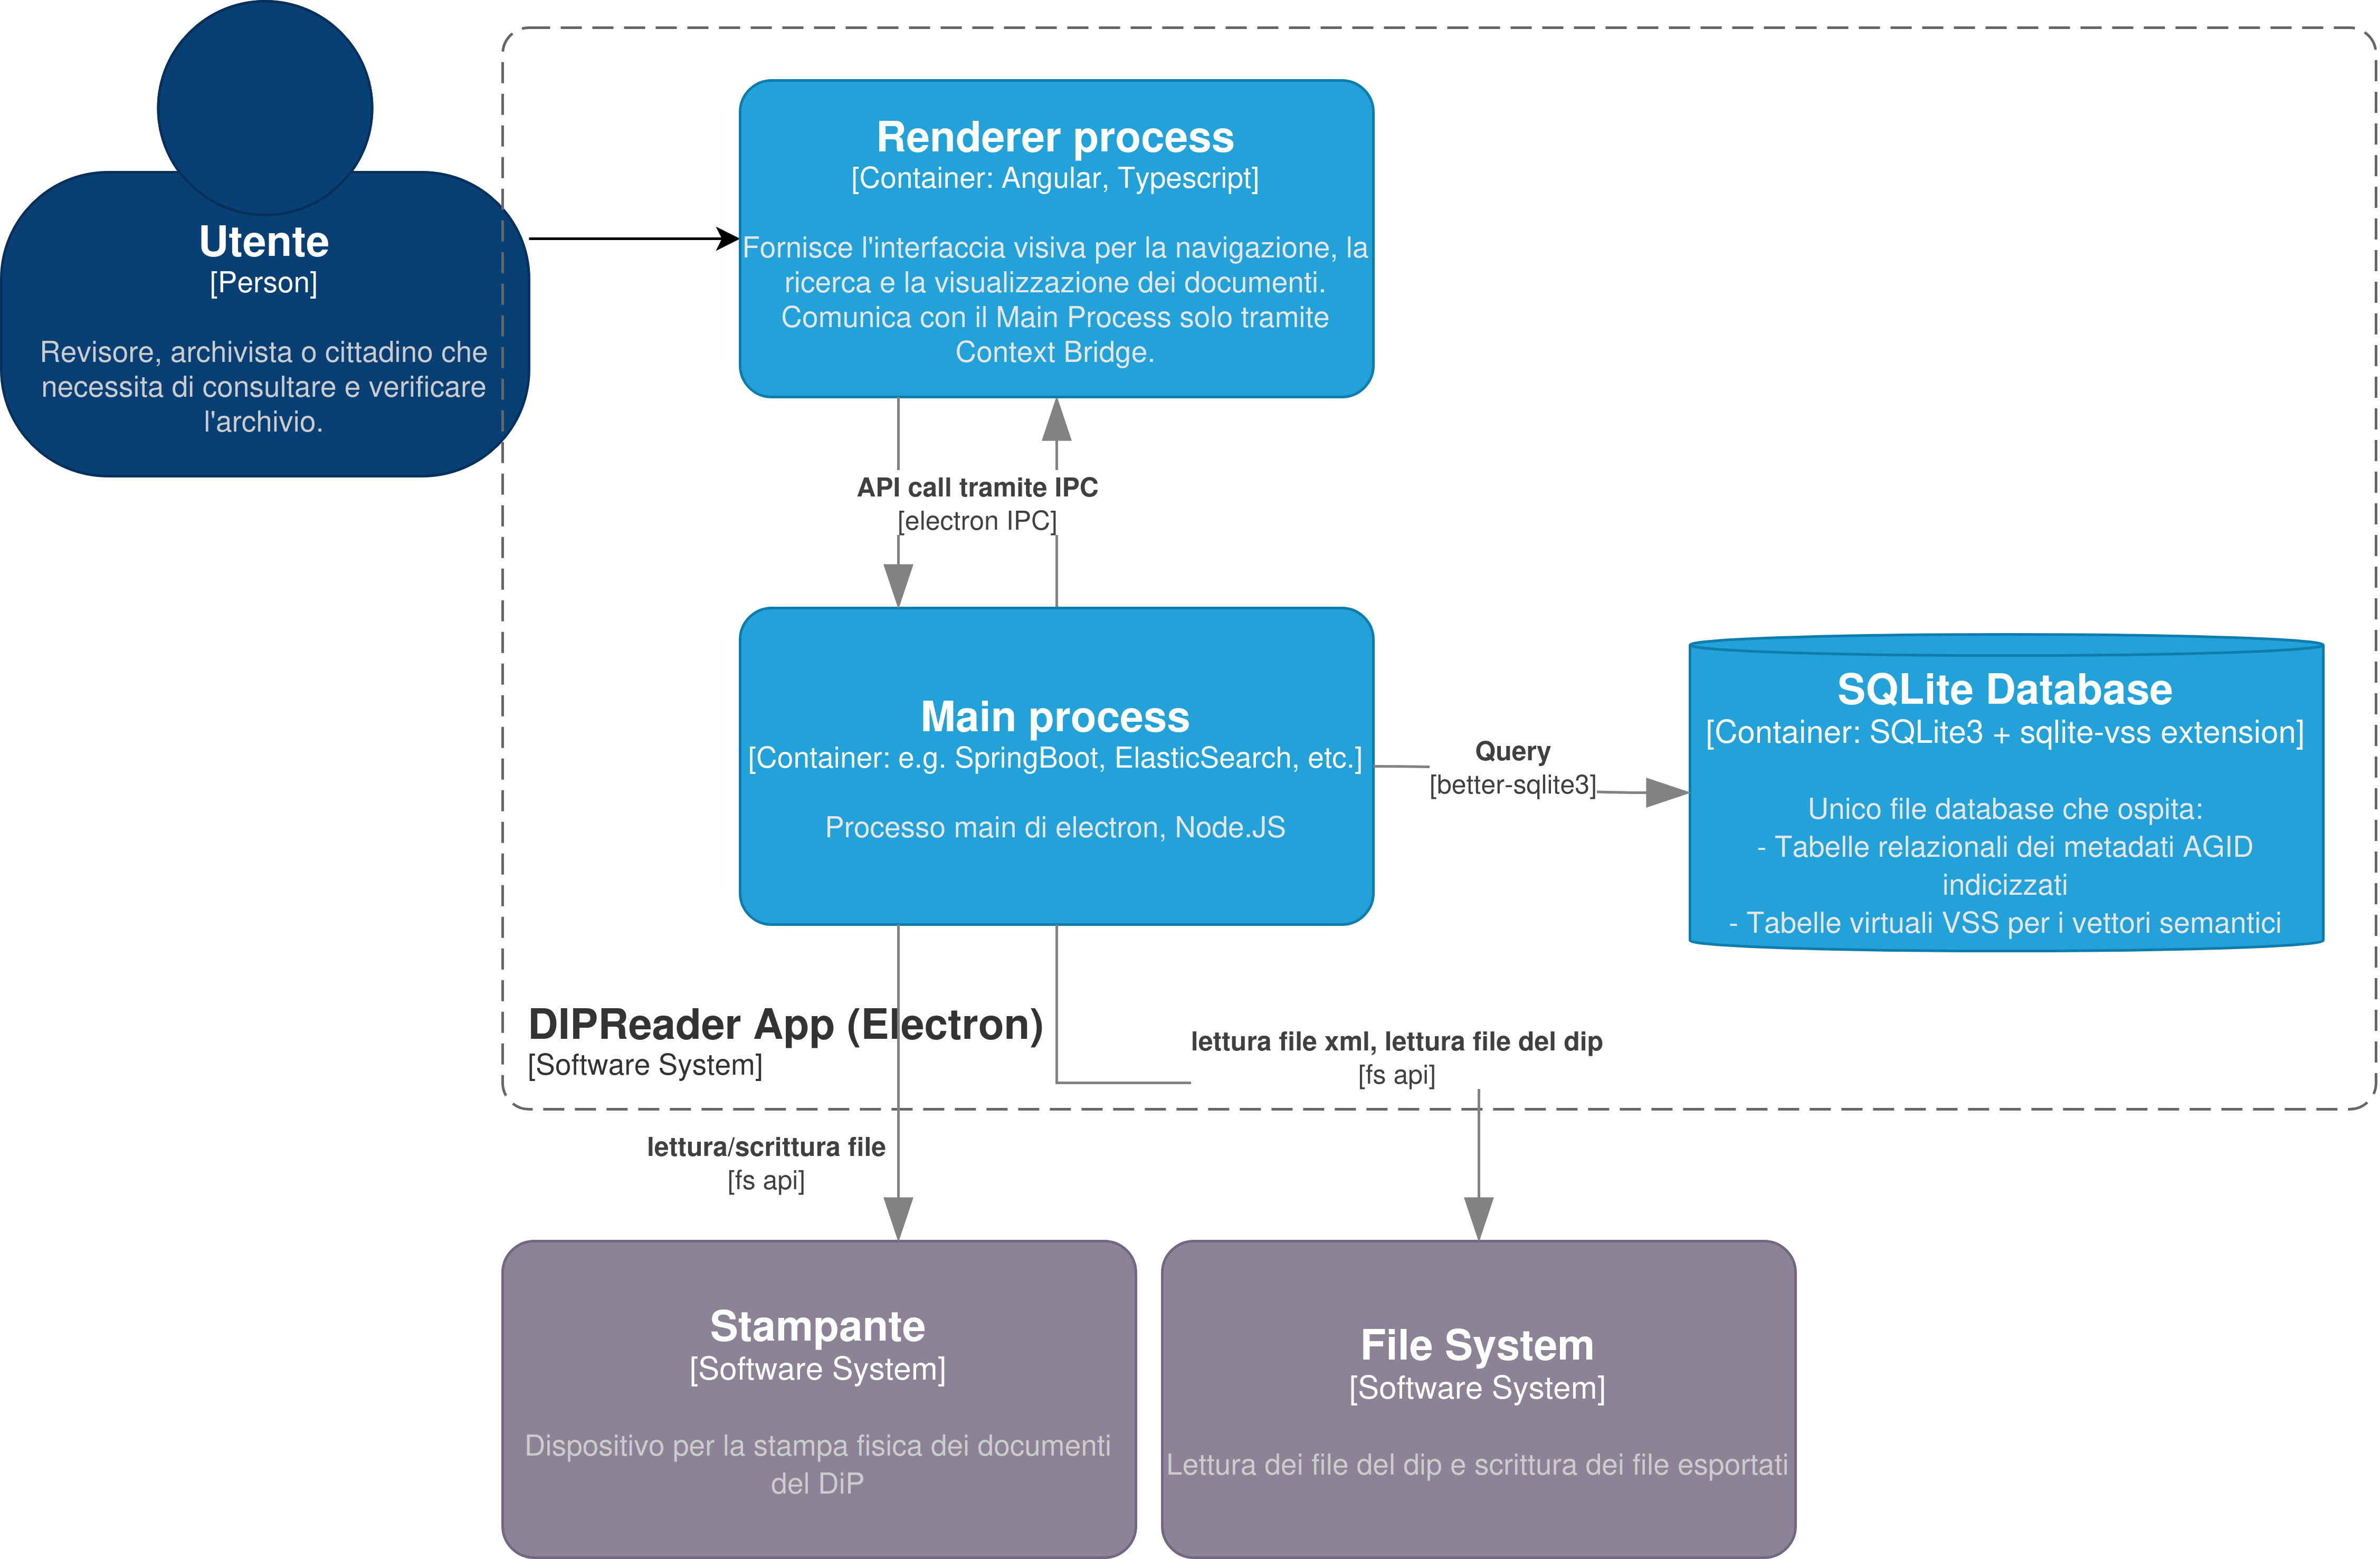
\includegraphics[width=1\textwidth]{../../assets/outDiagrammiST/DiagrammaC2(1).png}
        \caption{Diagramma C2 - Container del sistema \textit{DIPReader}}
    \label{fig:C2_container}
\end{figure}

\subsection{Renderer}
\subsubsection{Struttura architetturale}
Il container \textit{Renderer} è responsabile della presentazione dell'interfaccia utente e dell'interazione con l'utente. 
Il processo renderer ospita l'applicazione Angular, eseguita dal motore Chromium di Electron. Il frontend è sviluppato come SPA (Single Page Application) e segue un'architettura a componenti, con una chiara separazione tra logica di presentazione e logica di coordinamento. È inoltre applicato il pattern Smart and Dumb Components, che separa la logica di orchestrazione dalla presentazione pura.\\
Infine, essendo l'applicazione sviluppata in Angular, adotta il pattern MVVM (Model View ViewModel) per la gestione della UI.
\subsubsection{Relazione con i principi SOLID}
\begin{itemize}
    \item \textbf{SRP:} ogni componente ha una sola responsabilità.
    \item \textbf{OCP:} nuovi componenti possono essere aggiunti estendendo i contratti esistenti.
    \item \textbf{LSP e ISP:} i layer dipendono da interfacce coese e sostituibili. 
    \item \textbf{DIP:} Sono iniettati i token delle interfacce dei servizi, non le implementazioni concrete.
\end{itemize}

\subsection{Main}
\label{sec:container:main}

\subsubsection{Ruolo architetturale}
Il container \textit{Main} ospita la logica backend e costituisce il punto di orchestrazione tra IPC, use case applicativi e persistenza su SQLite.
Le responsabilita principali sono la registrazione degli handler IPC, l'implementazione della business logic e il bootstrap iniziale dei dati indicizzati.
In particolare, l'architettura del main process è stata organizzata in maniera tale da definire solamente le entità di un pacchetto DiP, gestendo invece i metadati in maniera generica. Questo permetterà in un futuro di evolvere il sistema per supportare nuovi tipi di schema di metadati, senza dover modificare o aggiungere nessuna componente o entità al backend.

\subsubsection{Layer architetturali}
\begin{enumerate}
    \item \textbf{IPC Adapter:} boundary verso renderer, gestione canali, mapping DTO.
    \item \textbf{Use Case:} business logic layer, utilizza servizi e porte outbound per ottenere il risultato.
    \item \textbf{Outbound port:} layer di astrazione per l'interazione con servizi esterni.
    \item \textbf{Outbound adapter:} implementazione concreta delle porte verso p.e. database o filesystem.
    \item \textbf{DAO:} query SQL concrete, ricostruzione entity da righe.
    \item \textbf{Mapper:} trasformazione DTO $\leftrightarrow$ Entity $\leftrightarrow$ Persistence.
    \item \textbf{Entity / Value Objects:} modello di dominio.
\end{enumerate}

\subsubsection{Relazione con i principi SOLID}
\begin{itemize}
    \item \textbf{SRP:} ciascun componente ha un solo motivo per cambiare: ciascuna classe ha una responsabilità ben definita e limitata. Sinonimo di coesione: un classe è coesa se le classi client che la utilizzano usano tutti i metodi della classe.
    \item \textbf{OCP:} nuovi use case o adapter possono essere aggiunti estendendo i contratti esistenti.
    \item \textbf{LSP e ISP:} i layer dipendono da interfacce coese e sostituibili.
    \item \textbf{DIP:} le concretizzazioni (adapters) dipendono da astrazioni (porte), non viceversa.
\end{itemize}

\subsubsection{Bootstrap e indicizzazione}
\noindent
\textbf{DatabaseBootstrap.ts} (avvio):
\begin{enumerate}[labelwidth=0.8cm,leftmargin=1cm]
    \item Ricrea database zero.
    \item Applica schema.
    \item Chiama \codeword{IndexDip.execute(dipPath)}.
\end{enumerate}

\subsubsection{Wiring runtime e registrazioni}
\noindent
Durante l'avvio dell'applicazione electron, \codeword{main.ts} esegue:

\begin{enumerate}[labelwidth=0.8cm,leftmargin=1cm]
    \item bootstrap database tramite \codeword{ApplicationBootstrapAdapter}
    \item registrazione token runtime \codeword{DIP\_PATH\_TOKEN}
    \item registrazione adapter IPC (es. \codeword{BrowsingIpcAdapter}, \codeword{CheckIntegrityIpcAdapter})
\end{enumerate}
\newpage
\section{Architettura delle componenti}

\subsection{[Componente 1]}
    \subsubsection{Descrizione}
    \subsubsection{Interfacce}
    \subsubsection{Dipendenze} %da vedere se ha senso tenerlo
    \subsubsection{Tracciamento dei requisiti}

\subsection{[Componente 2]}
    \subsubsection{Descrizione}
    \subsubsection{Interfacce}
    \subsubsection{Dipendenze} %da vedere se ha senso tenerlo
    \subsubsection{Tracciamento dei requisiti}

\newpage
\subsection{Componenti di Verifica Integrità (Frontend)}
\subsubsection{Descrizione}
La funzionalità di verifica integrità garantisce la correttezza e l'autenticità dei pacchetti DIP, verificando ricorsivamente l'integrità crittografica (generalmente hash SHA-256) dei file contenuti, propagando poi il risultato alla gerarchia documentale.

Per gestire l'albero delle dipendenze documentali sono stati adottati diversi design patterns:
\begin{itemize}
    \item \textbf{Facade Pattern}: tutta la logica dello state management è isolata in \textit{integrity.facade.ts}. In questo modo la facade agisce come single-source-of-truth per tutti i componenti di UI, inoltre coordina le chiamate ai servizi e gestisce lo stato interno \textit{isVerifying} e di invalidazione della cache quando necessario.
    \item \textbf{Angular Signals}: Angular contribuisce con il suo sistema di state management reattivo basato su Signals
\end{itemize} % Verifica Integrità
\subsection{Componenti di Ricerca (FrontEnd)}
\subsubsection{Descrizione}
I componenti di ricerca sono responsabili della gestione delle funzionalità di compilazione dei campi di ricerca.
\\ Come già anticipato il pattern applicato è quello di Smart and Dumb Components, per cui i componenti di ricerca sono suddivisi in componenti di pura presentazione e gestiti da i componenti \textit{"Padri"}, che si occupano di gestire la logica di questi ultimi nonchè le interazioni con altri servizi come la validazione dei filtri, la gestione dei campi di ricerca dinamici e il routing della sezione dei risultati.
Nel contesto della ricerca questo coomponente Padre è SearchPageComponent.
% FOTO SCHEMA SEARCHPAGE COMPONENT

Come si può notare questo componente sfrutta la dependency injection nativa di Angular per risolvere le dipendenze. 
Inoltre sono iniettate le interfaccie dei servizi necessari per il funzionamento e non gli effettivi servizi, applicando il principio di sostituzione di Liskov. 
La page si appoggia poi alla SearchFacade per gestire tutte le interazioni con i servizi, nascondendo la complessità di questi ultimi e fornendo un'interfaccia semplificata per la gestione della logica di ricerca.

\subsubsection{Componenti di presentazione} 
I componenti di presentazione pura sono costruiti in modo da adattarsi completamente alle specifiche descritte dall'Allegato 5 dell'AGID e dalle linee guida di Sanmarco Informatica.
\\ Posso essere suddivisi in tre categorie principali:
\begin{itemize}
    \item \textbf{Componenti di ricerca}: sono i componenti che gestiscono la compilazione dei filtri di ricerca.
    \item \textbf{Componenti di visualizzazione}: sono i componenti che gestiscono la visualizzazione dei risultati di ricerca.
    \item \textbf{Search bar}: è il componente che si occupa della ricerca di processi, classi documentali e ricerca semantica.
\end{itemize}
\paragraph{Componenti di ricerca}
\subparagraph{AdvancedFilterPanelComponent}
I diversi filtri di ricerca, basati sui metadati AGID, sono raggruppati nel \textit{AdvancedFilterPanelComponent}. Anche in questo caso le dipendenze sono risolte grazie alla dependency injection di Angular. 
La responsabilità di questo componente è quella di gestire la compilazione dei filtri fi ricerca, delegando le logiche secondarie ai servizi iniettati.
In particolare, è iniettata l'interfaccia del servizio di validazione dei filtri, che si occupa di validare i filtri di ricerca dinamici, e il servizio di gestione dei campi di ricerca dinamici, che si occupa di gestire i campi di ricerca dinamici.\\
\subparagraph{FilterRulesManager}
La gestione dei campi di ricerca risulta infatti fondamentale per garantire che la query di ricerca sia sensata. Dal momento che i campi sono differenti a seconda del tipo di documento, è obbligatorio forzare l'utente a compilare solo i campi di ricerca pertinenti al tipo di documento. Questo compito è delegato al \textit{FilterRulesManager}. 
\subparagraph{Filtri semplici}
La maggior parte dei filtri di ricerca sono semplici campi di testo o dropdown, che non richiedono una logica complessa per la loro gestione. Segue quindi un elenco di questi componenti di UI pura, al fine di mostrare la completa aderenza alle specifiche AGID e alle linee guida di Sanmarco Informatica.
\begin{itemize}
    \item \textit{CommonFiltersComponent}: è il componente che gestisce i filtri comuni a tutti i tipi di documento (Anni di Conservazione, Chiave descrittiva, Classificazione con i corrispettivi sottocampi) 
    \item \textit{DiDaiFiltersComponent}: è il componente che gestisce i filtri specifici per i documenti informatici e amministrativi informatici (tipologia di documento, modalità di formazione, Nome, versione id del documento, informazioni sull'identificativo di formato, dati di veriffica e tracciatura con riguardo alla tracciatura delle modifiche)
    \item  \textit{AggregateFiltersComponent}: è il componente che gestisce i filtri specifici per le aggregazioni documentali (tipologia e id di aggregazione, data di apertura e chiusura, dati di procedimento e delle sue fasi e dati sulle assegnazioni)
\end{itemize}
\subparagraph{Filtri dei soggetti}
I filtri dei soggetti sono invece più complessi. La loro gestione è realizzata secondo un approccio a strategie, così da rendere il comportamento dell'interfaccia dipendente dal contesto documentale selezionato e non da logiche condizionali distribuite nel codice.
 Il sistema consente di abilitare, disabilitare e specializzare i criteri disponibili in funzione del tipo di documento, mantenendo separati gli aspetti di presentazione, configurazione delle regole e costruzione della query.
\\
L'interazione dell'utente avviene attraverso il pannello dei filtri avanzati, che funge da contenitore dello stato complessivo e coordina i diversi sotto-filtri. 
All'interno di tale pannello, il componente dedicato ai soggetti gestisce un wizard guidato: in base al DocContext viene selezionata, tramite una registry di strategie, la configurazione dei ruoli consentiti e dei relativi tipi di soggetto. 
Una seconda registry definisce invece i campi di dettaglio associati a ciascun SubjectType, consentendo la generazione dinamica del form di compilazione.

I criteri inseriti vengono raccolti come \textit{SubjectCriteria} e successivamente integrati nello stato complessivo dei filtri. In fase di esecuzione della ricerca, tali valori vengono trasformati in una struttura di query gerarchica 
compatibile con il back-end, così da mantenere una separazione netta tra modello di interfaccia e modello di ricerca. Questo consente di garantire coerenza funzionale, facilità di estensione e una più chiara manutenzione delle regole di validazione e composizione dei filtri.

\subparagraph{Filtri Custom}
I filtri custom sono metadati personalizzati di un documento costituiti da una chiave e un valore. Per soddisfare la richiesta dell''azienda proponente di esporre all'utente una lista di chiavi che rappresenta quelle effettivamente presenti nei documenti, è stato realizzato un componente 

\paragraph{Componenti di visualizzazione}
La visualizzazione dei risultati di ricerca deve rendere possibile la visualizzazione all'utente di anteprime di processi, classi, aggregazioni e documenti. Queste visualizzazioni sono naturalmente diverse. Per esempio solo i documenti possono essere stampati o scaricati. Le informazioni mostrate per i processi sono invece differenti da quelle mostrate per i documenti e dalle classi.
\\La necessità è quindi quella di mostrare in modo dinamico i risultati di ricerca in base al tipo di risultato che viene ritornato. Per questo motivo è stato scelto di sfruttare un pattern \textit{Factory}.
\\ il \textit{SearchResultFactory} si occupa di istanziare dinamicamente il componente di visualizzazione corretto in base al tipo di risultato di ricerca sfruttando un registry che associa al tipo di risultato il componente di visualizzazione corrispondente. 
\paragraph{Search bar}
La  % Search 
\subsection{Componenti di Dettaglio (Frontend)}
\subsubsection{Descrizione}
All'interno di DIPReader la feature di dettaglio rappresenta il cuore della consultazione. Poiché un DIP aderisce allo standard OAIS, le entità che lo compongono all'interno dell'albero hanno una struttura ben definita non sempre trasversale a tutte le entità: processi, documenti informatici, documenti amministrativi informatici, aggregazioni documentali e le classi documentali che fungono da contenitori logici. La feature di dettaglio è quindi composta da più componenti, ognuna dedicata alla visualizzazione di una specifica entità, che condividono però un'interfaccia comune per poter essere utilizzata in modo intercambiabile all'interno dell'albero.\\

Invece di duplicare le pagine di routing per ogni entità quindi è stata sviluppata la feature \textit{Item-Detail} per sfruttare una singola rotta generica \textit{/detail/:itemType/:itemId} che, a seconda del tipo di entità e dell'identificativo, renderizza il componente specifico per quella entità. Questo approccio implementa un design pattern di tipo strategy con polimorfismo statico, in cui la logica di selezione dell'entità da visualizzare è centralizzata e ben definita grazie alla tipizzazione statica di TypeScript, la scelta è stata dettata dalla considerazione che la struttura dei dati è ben definita e non si prevede l'aggiunta di nuovi tipi di entità in futuro, la possibilità di estensione riguarda invece i metadati delle entità.

\subsubsection{Componente principale}
Il componente principale della feature è \textit{ItemDetailPageComponent}, che agisce da orchestratore e si occupa di:
\begin{itemize}
    \item multiplexing dei Token delle facade delle singole entità e indirizzamento alla facade corretta, con un componente di fallback per coprire i casi di entità vuote come le classi documentali;
    \item adattamento del layout grafico a seconda del tipo di entità, per i documenti viene utilizzato un layout comprensivo di un'anteprima del file, mentre per aggregazioni e processi viene mostrato un indice dei documenti che li compongono;
\end{itemize}

\subsubsection{Componente dei metadati}
Il componente \textit{MetadataPanelComponent} decide quali componenti di metadati visualizzare in base al tipo di entità selezionata. Esso intercetta i dati passati dall'interfaccia dell'entità da visualizzare e in base ad essa decide quali componenti mostrare. Ad esempio, per i documenti sono presenti i componenti relativi alle informazioni del processo di conservazione, degli allegati, del formato del file, dei metadati custom, ecc., mentre per le aggregazioni e i processi vengono mostrati oltre ai metadati anche gli indici dei documenti che li compongono.

\subsubsection{Componente di azioni sugli elementi}
Il componente \textit{DocumentActionsComponent} crea la barra orizzontale di azioni che è possibile eseguire su un'entità, per tutte offre la verifica dell'integrità, per i documenti è anche possibile scaricarli o stamparli tramite il componente della feature di Export.

\subsubsection{Componenti specifici per entità - DOCUMENT}
È il modulo più denso di informazioni, ospita una notevole quantità di componenti \textit{dumb} per le sezioni specifiche dei metadati OAIS e i componenti per la visualizzazione dell'anteprima.

\subparagraph{DocumentViewerComponent}
Il componente \textit{DocumentViewerComponent} è responsabile della visualizzazione dell'anteprima del documento, supporta i formati PDF, XML, JPEG, PNG e testo semplice. Se il formato del documento non è supportato, interviene la logica di gestione degli errori unificata che restituisce un \textit{AppError}.

\subparagraph{Schede metadati}
Ogni sottoinsieme dei metadati nel formato XML viene visualizzato in un componente dedicato:
\begin{itemize}
    \item \textit{document-metadata}: identificativo, livello di riservatezza, hash del documento;
    \item \textit{aip-info}: fornisce le proprietà di storicizzazione a lungo termine e riporta le informazioni di conservazione a norma;
    \item \textit{attachments}: mostra l'elenco degli allegati associati al documento, con la relativa impronta crittografica;
    \item \textit{change-tracking}: proprietà di versionamento;
    \item \textit{classification-info}: restituisce l'indice e il piano di classificazione secondo i registri della PA;
    \item \textit{format-info}: mostra il formato MIME del documento;
    \item \textit{registration-data}: mostra i dati di registrazione del documento, sia protocollato che non protocollato;
    \item \textit{subject-list}: mostra i soggetti coinvolti nella produzione del documento, con i relativi ruoli;
    \item \textit{verification-info}: mostra i risultati dell'ultima verifica di integrità eseguita sul documento;
    \item \textit{custom-metadata}: mostra i metadati custom definiti dall'ente, con un formato standard chiave-valore.
\end{itemize}

\subparagraph{Interfacce/Dominio/Servizi/Mappers}
Come per tutte le feature, sono presenti le interfacce per i servizi, i servizi stessi, i mappers per adattare i dati restituiti dal backend al formato utilizzato dai componenti e le interfacce per i DTO estrate dagli schema XSD forniti e dalla documentazione AGID sui metadati. \\
Rimangono rispettati quindi i principi di separazione dei compiti, single responsibility e inversion of control.

\subsubsection{Componenti specifici per entità - AGGREGATE}
I componenti dedicati alla visualizzazione di aggregazioni e processi sono più semplici rispetto a quelli dei documenti, in quanto non prevedono l'anteprima del file e hanno una quantità inferiore di metadati da visualizzare.  % Document Details
%\input{specifica/F-AD.tex} % Aggregate Details 
%\newpage
\section{Componente Frontend: Modulo Export}

\subsection{Descrizione}
Il modulo Export gestisce l'\textit{application logic} dedicata all'estrazione, salvataggio e stampa dei documenti contenuti nei pacchetti di archiviazione. Il modulo coordina le operazioni di trasferimento dei file dal sistema protetto (DIP) verso il \textit{file system} locale dell'utente o verso le periferiche di output. L'architettura segue il pattern Smart-Dumb Components per la gestione dei progressi di scaricamento e il pattern Facade per l'orchestrazione delle richieste IPC.

\subsubsection{Lista delle Classi e Strutture Dati}

\paragraph{ExportState}
Oggetto responsabile della gestione dello stato reattivo delle operazioni di output tramite Angular Signals. Traccia il ciclo di vita delle richieste di esportazione e la persistenza temporanea dei risultati.

\paragraph{Descrizione degli attributi della struttura:}
\begin{itemize}
\item \textbf{phase Signal}: segnale che rappresenta lo stato globale dell'operazione (IDLE, EXPORTING, COMPLETED, ERROR);
\item \textbf{progress Signal}: valore numerico (0-100) che indica la percentuale di avanzamento dell'operazione di esportazione corrente;
\item \textbf{lastResult Signal<ExportResult | null>}: memorizza l'esito dell'ultima operazione (es. percorso di salvataggio, numero di file estratti);
\item \textbf{error Signal<AppError | null>}: contiene l'eventuale errore riscontrato durante la comunicazione IPC o l'accesso al disco;
\item \textbf{loading Signal}: indica se il modulo è in attesa di una risposta dal processo Main per un'operazione di I/O.
\end{itemize}

\paragraph{Descrizione dei metodi invocabili dalla struttura:}
\begin{itemize}
\item \textbf{setExporting()}: imposta la fase su EXPORTING e resetta il progresso;
\item \textbf{updateProgress(value: number)}: aggiorna il segnale del progresso durante i download multipli;
\item \textbf{setSuccess(result: ExportResult)}: imposta lo stato su COMPLETED e memorizza i dettagli dell'esito;
\item \textbf{setError(error: AppError)}: registra un fallimento critico (es. permessi disco negati);
\item \textbf{reset()}: riporta il modulo allo stato IDLE.
\end{itemize}

\paragraph{ExportFacade}
Implementa la \textit{business logic} di coordinamento per le funzionalità di output. Funge da interfaccia unificata per i componenti della UI (\textit{ExportPage}, \textit{ExportProgress}) delegando le chiamate di sistema all'infrastruttura. Implementa l'interfaccia \textit{IExportFacade}.

\paragraph{Descrizione degli attributi della struttura:}
\begin{itemize}
\item \textbf{exportState ExportState}: istanza del servizio di gestione dello stato reattivo delle esportazioni;
\item \textbf{ipcGateway ExportIpcGateway}: istanza del gateway incaricato di dialogare con i canali di download di Electron.
\end{itemize}

\paragraph{Descrizione dei metodi invocabili dalla struttura:}
\begin{itemize}
\item \textbf{exportDocument(documentId string) Promise}: avvia la procedura di salvataggio per un singolo documento. Gestisce l'apertura della finestra di dialogo nativa tramite gateway e monitora l'esito;
\item \textbf{exportMultiple(documentIds string[]) Promise}: coordina l'estrazione massiva di documenti, aggiornando progressivamente lo stato di avanzamento per ogni file processato;
\item \textbf{printDocument(documentId string) Promise}: invoca il servizio di sistema per la stampa diretta del documento selezionato;
\item \textbf{cancelOperation() void}: tenta di interrompere un'operazione di esportazione in corso tramite segnale IPC.
\end{itemize}

\paragraph{Descrizione dei segnali esposti:}
\begin{itemize}
\item \textbf{progress}: espone l'avanzamento percentuale per la UI;
\item \textbf{phase}: permette alla UI di reagire al cambio di stato (es. mostrando lo spinner o il messaggio di successo);
\item \textbf{lastResult}: fornisce i metadati dell'operazione conclusa.
\end{itemize}

\subsection{Interfacce}

\subsubsection{IExportFacade}
Definisce il contratto per la Business Logic del modulo Export. Stabilisce i metodi necessari per le azioni di output e i segnali per il monitoraggio dei processi asincroni.

\paragraph{Descrizione dei metodi dell'interfaccia:}
\begin{itemize}
\item \textbf{exportDocument(id: string) Promise}: contratto per l'estrazione singola;
\item \textbf{exportMultiple(ids: string[]) Promise}: contratto per l'estrazione di gruppo;
\item \textbf{printDocument(id: string) Promise}: contratto per l'invio alla periferica di stampa.
\end{itemize}

\subsubsection{IExportChannel}
Interfaccia di contratto per il layer di infrastruttura. Definisce le firme per le chiamate IPC dedicate ai flussi di file tra il sandbox di Electron e il sistema operativo.

\paragraph{Descrizione dei metodi dell'interfaccia:}
\begin{itemize}
\item \textbf{saveFile(id: string) Promise}: definisce la richiesta di apertura del \textit{Save Dialog} nativo;
\item \textbf{print(id: string) Promise}: definisce la richiesta di stampa;
\item \textbf{openFolder(path: string) void}: comando per aprire la cartella di destinazione nel file manager di sistema.
\end{itemize}

\subsubsection{ExportIpcGateway}
Adapter di infrastruttura che implementa la comunicazione asincrona verso i canali \texttt{file:*} di Electron. Utilizza il bridge fornito dal contesto di esecuzione desktop.

\paragraph{Descrizione dei metodi invocabili dalla struttura:}
\begin{itemize}
\item \textbf{saveFile(id string)}: invoca il canale \texttt{file:download-single} passando l'identificativo del documento e riceve il percorso finale scelto dall'utente;
\item \textbf{print(id string)}: esegue l'invocazione del canale \texttt{file:print-document};
\item \textbf{requestMultiExport(ids string[])}: inizializza una sessione di esportazione massiva sul canale \texttt{file:download-batch}.
\end{itemize}

\subsection{Dipendenze}
\begin{itemize}
\item \textbf{Angular Signals}: gestione della reattività del progresso e degli stati di errore;
\item \textbf{Electron IPC Bridge}: per l'accesso alle \textit{Native APIs} del sistema operativo (File System e Print Manager);
\item \textbf{Domain Models/DTOs}: definizioni condivise per rappresentare i risultati dell'esportazione (\textit{ExportResult}) e i metadati di trasporto.
\end{itemize}

\subsection{Tracciamento dei requisiti}
La tabella seguente mappa i requisiti funzionali obbligatori relativi all'Export sulle componenti realizzate.

\begin{table}[H]
    \centering
    \begin{tabular}{|p{2.5cm}|p{6.5cm}|p{5.5cm}|}
        \hline
        \rowcolor{zpusgreen!30}
        \textbf{Codice} & \textbf{Descrizione Sintetica} & \textbf{Componente Software} \\
        \hline
        \textbf{R-178-F-Ob} & Salvataggio di un documento in locale. & \textit{ExportFacade, ExportIpcGateway} \\
        \hline
        \textbf{R-179-F-Ob} & Salvataggio multiplo di documenti. & \textit{ExportFacade, ExportProgress} \\
        \hline
        \textbf{R-181-F-Ob} & Stampa di un documento. & \textit{ExportFacade, ExportIpcGateway} \\
        \hline
        \textbf{R-224-F-Ob} & Selezione della cartella di destinazione. & \textit{IExportChannel, ExportPage} \\
        \hline
        \textbf{R-226-F-Ob} & Protezione della cartella sorgente del DIP. & \textit{ExportFacade (Business Logic)} \\
        \hline
    \end{tabular}
    \caption{Tracciamento Requisiti Funzionali - Modulo Export}
\end{table}  % Import 
\subsection{Componenti di Navigazione (Frontend)}

\subsubsection{Descrizione}
Il modulo di navigazione realizza l'albero gerarchico del DIP ed e il punto di ingresso principale per la consultazione delle entita archivistiche. La gerarchia visualizzata segue il modello:
\begin{center}
DIP -> DocumentClass -> Process -> Document -> File
\end{center}

L'implementazione segue una separazione netta delle responsabilita:
\begin{itemize}
	\item \textbf{Facade Pattern}: \textit{DipFacade} coordina stato, caricamenti e retry.
	\item \textbf{Gateway Pattern}: \textit{IpcGateway} incapsula la comunicazione IPC con il backend.
	\item \textbf{Smart/Dumb Components}: componenti smart per orchestrazione, componenti dumb per sola presentazione del nodo.
	\item \textbf{State reattivo}: la UI reagisce ai cambiamenti di stato di root, cache, loading e errori locali.
\end{itemize}

\subsubsection{Diagrammi condivisi (C1/C2/C3)}

\begin{figure}[H]
	\centering
	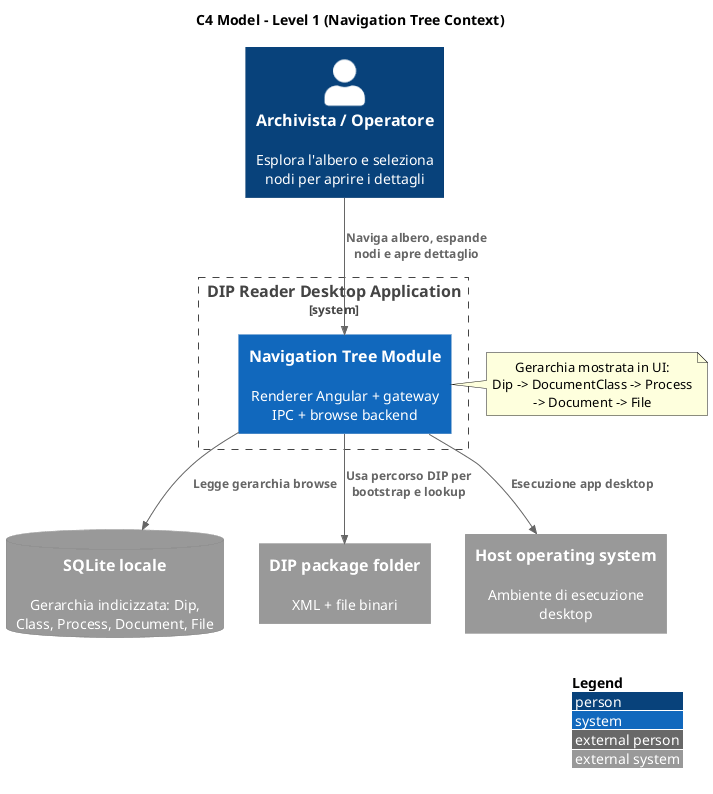
\includegraphics[width=0.85\textwidth]{../../assets/outDiagrammiST/C4_Navigation_Context.png}
	\caption{Diagramma C1 - System Context del modulo Albero di Navigazione}
	\label{fig:navigation:c1-context}
\end{figure}

\begin{figure}[H]
	\centering
	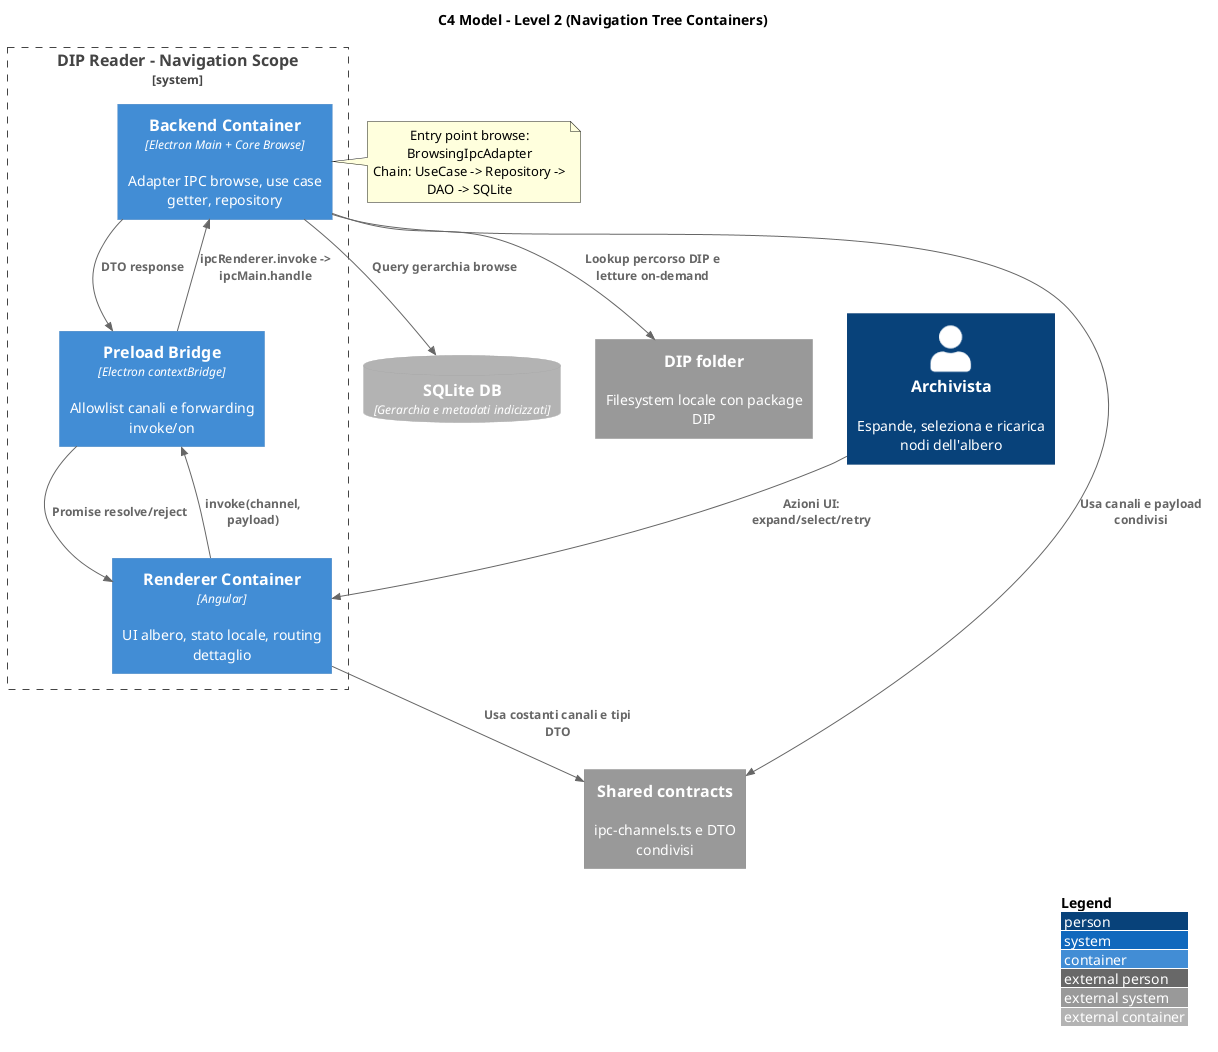
\includegraphics[width=0.85\textwidth]{../../assets/outDiagrammiST/C4_Navigation_Container.png}
	\caption{Diagramma C2 - Container View del modulo Albero di Navigazione}
	\label{fig:navigation:c2-container}
\end{figure}

\begin{figure}[H]
	\centering
	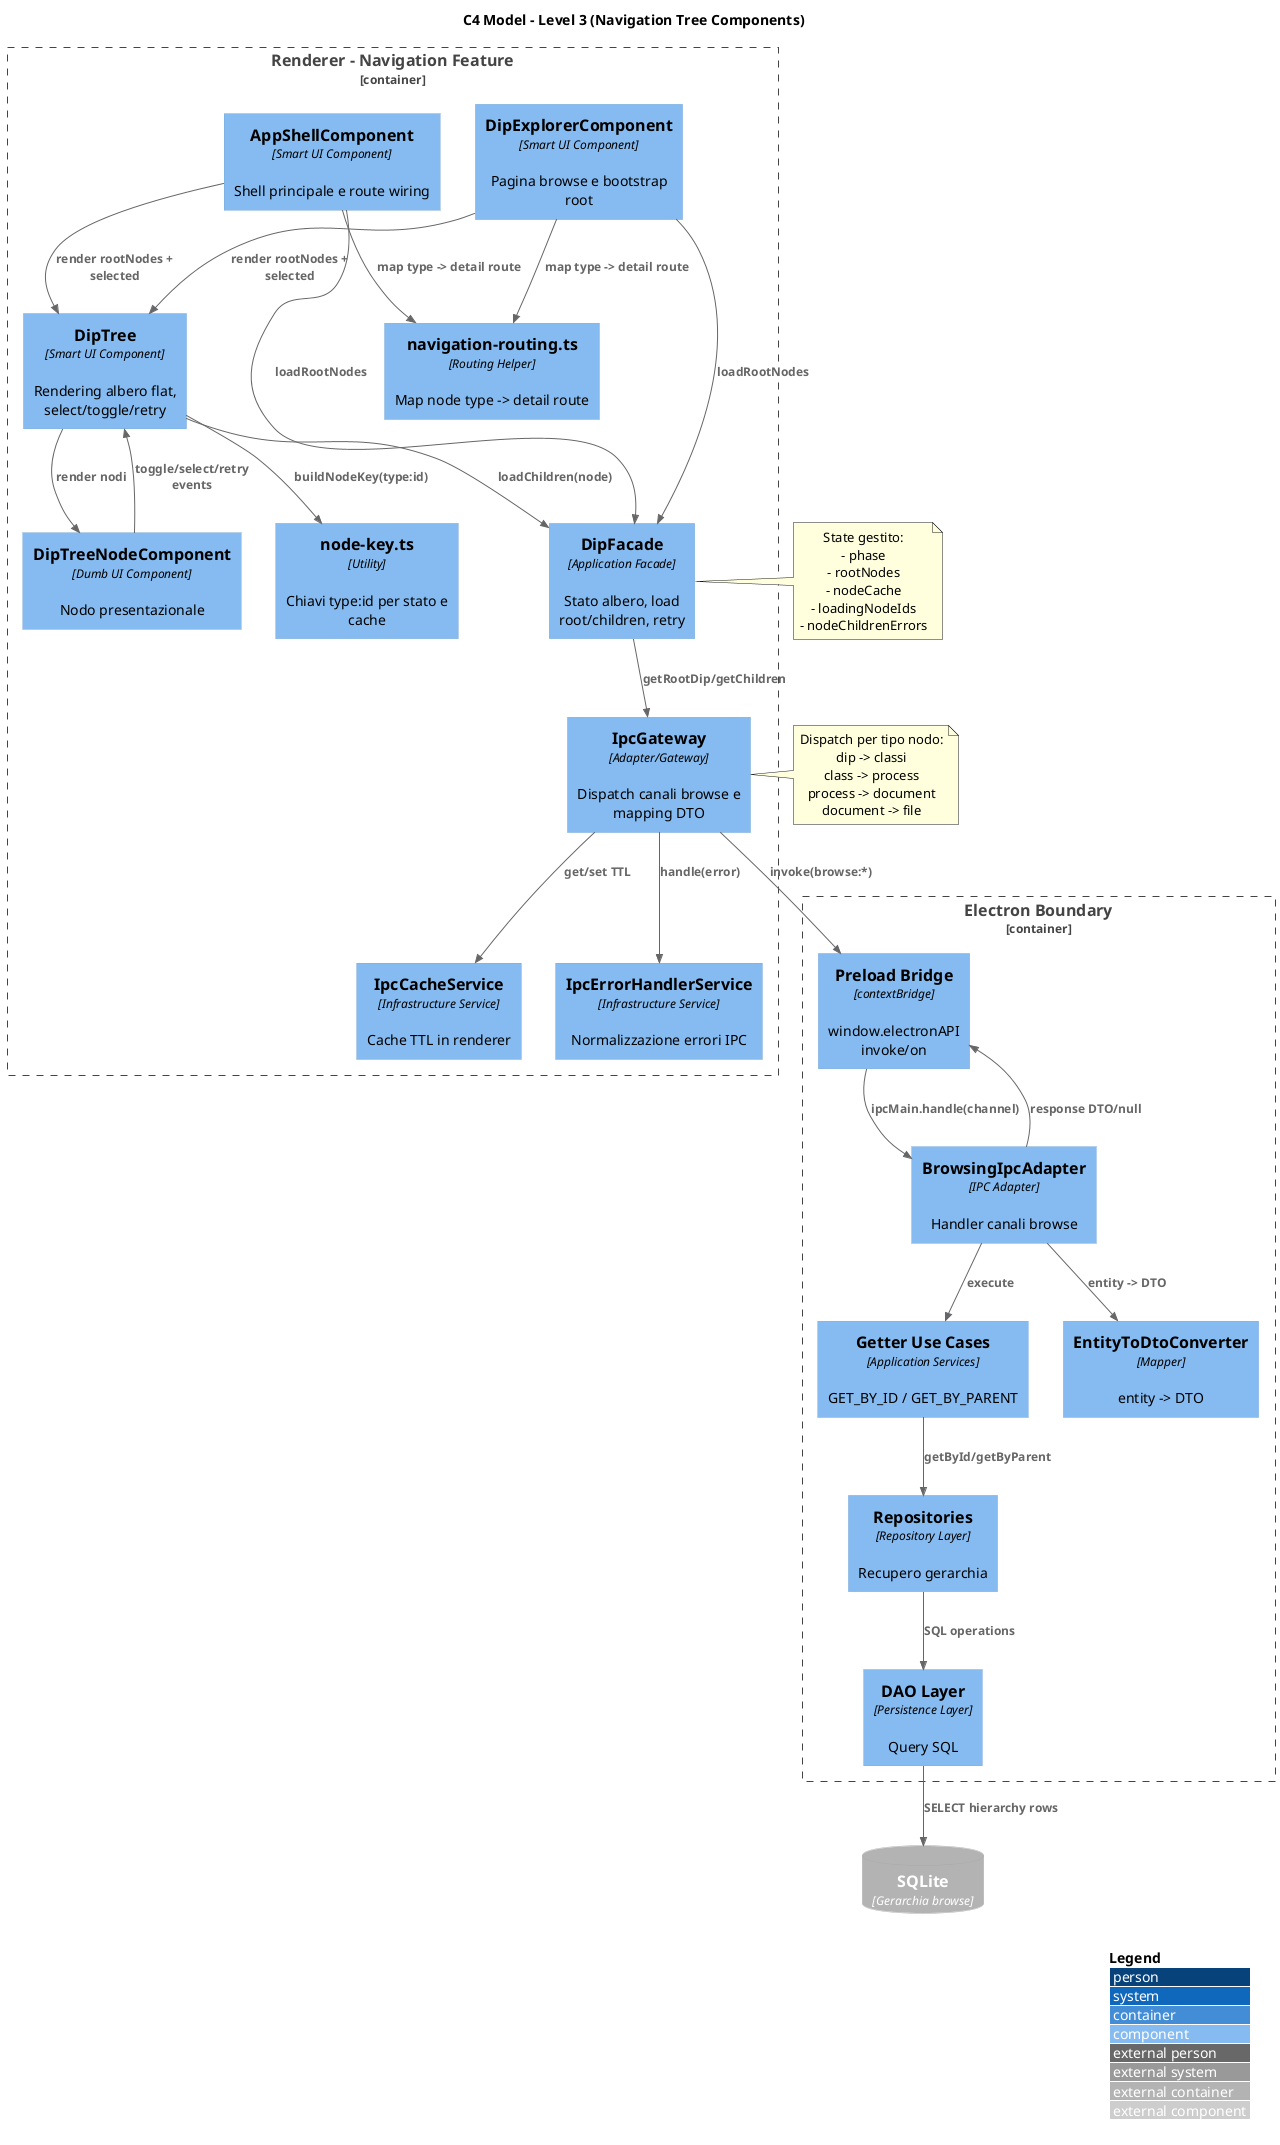
\includegraphics[width=0.9\textwidth]{../../assets/outDiagrammiST/C4_Navigation_Component.png}
	\caption{Diagramma C3 - Component View del modulo Albero di Navigazione}
	\label{fig:navigation:c3-component}
\end{figure}

\subsubsection{Architettura del modulo}

\begin{table}[H]
	\centering
	\footnotesize
	\setlength{\tabcolsep}{4pt}
	\renewcommand{\arraystretch}{1.35}
	\begin{tabularx}{\textwidth}{|l|l|Y|}
		\hline
		\textbf{Layer} & \textbf{Componente} & \textbf{Responsabilita} \\
		\hline
		Renderer & \texttt{DipFacade} & Stato albero (phase, rootNodes, nodeCache, loadingNodeIds, nodeChildrenErrors), orchestrazione load root/children, retry e gestione errori. \\
		\hline
		Renderer & \texttt{IpcGateway} & Dispatch canali browse per tipo nodo, mapping DTO -> DipTreeNode, cache TTL, fallback naming. \\
		\hline
		Renderer & \texttt{DipTree} / \texttt{DipTreeNodeComponent} & Rendering albero flat, espansione/collasso, selezione nodo e retry locale. \\
		\hline
		Renderer & \texttt{AppShellComponent} / \texttt{DipExplorerComponent} & Bootstrap root nodes e integrazione con il routing di dettaglio. \\
		\hline
		Renderer & \texttt{navigation-routing.ts} / \texttt{node-key.ts} & Mapping tipo nodo -> route dettaglio e chiave composta \texttt{type:id} per cache/stato. \\
		\hline
		Backend & \texttt{preload.ts} / \texttt{main.ts} & Boundary Electron, allowlist canali, bridge invoke/on e registrazione adapter IPC. \\
		\hline
		Backend & \texttt{BrowsingIpcAdapter} + UseCase + Repository + DAO & Esecuzione query browse su SQLite e conversione entity -> DTO. \\
		\hline
	\end{tabularx}
	\caption{Architettura tecnica del modulo Navigazione}
	\label{tab:navigation:arch}
\end{table}

\subsubsection{Flussi operativi principali}

\paragraph{Bootstrap albero root}
\begin{enumerate}[labelwidth=0.8cm,leftmargin=1cm]
	\item \texttt{AppShellComponent} o \texttt{DipExplorerComponent} avvia l'inizializzazione dei nodi root.
	\item \texttt{DipFacade.loadRootNodes(dipId)} imposta \texttt{phase=loading}.
	\item \texttt{IpcGateway.getRootDip} invoca \texttt{BROWSE\_GET\_DIP\_BY\_ID}.
	\item Il backend risolve la richiesta via \texttt{BrowsingIpcAdapter} e catena UseCase -> Repository -> DAO.
	\item La facade aggiorna \texttt{phase=ready} e popola \texttt{rootNodes}.
\end{enumerate}

\paragraph{Espansione nodo}
\begin{enumerate}[labelwidth=0.8cm,leftmargin=1cm]
	\item \texttt{DipTree.toggleNode(node)} marca il nodo come espanso/collassato.
	\item Se il nodo non e in cache, \texttt{DipFacade.loadChildren(node)} avvia il caricamento.
	\item La facade aggiorna \texttt{loadingNodeIds} e pulisce eventuali errori pregressi sul nodo.
	\item \texttt{IpcGateway.getChildren} effettua dispatch per tipo nodo:
	\begin{itemize}
		\item dip -> \texttt{BROWSE\_GET\_DOCUMENT\_CLASS\_BY\_DIP\_ID}
		\item documentClass -> \texttt{BROWSE\_GET\_PROCESS\_BY\_DOCUMENT\_CLASS}
		\item process -> \texttt{BROWSE\_GET\_DOCUMENTS\_BY\_PROCESS}
		\item document -> \texttt{BROWSE\_GET\_FILE\_BY\_DOCUMENT}
		\item file -> nessun figlio
	\end{itemize}
	\item Al successo i figli sono salvati in \texttt{nodeCache}; al fallimento in \texttt{nodeChildrenErrors}.
\end{enumerate}

\paragraph{Selezione nodo e routing}
\begin{enumerate}[labelwidth=0.8cm,leftmargin=1cm]
	\item \texttt{DipTree.selectNode(node)} emette \texttt{nodeSelected}.
	\item AppShell/DipExplorer mappano il tipo nodo con \texttt{mapDipNodeTypeToDetailItemType()}.
	\item \texttt{buildDetailRoute(itemType, node.id)} costruisce la route target.
	\item Angular Router naviga verso \texttt{/detail/:itemType/:itemId}.
\end{enumerate}

\subsubsection{Contratti principali}

\paragraph{Stato della DipFacade}
\begin{itemize}
	\item \texttt{phase}: stato globale della feature (\texttt{ready|loading|idle}).
	\item \texttt{rootNodes}: nodi radice mostrati in albero.
	\item \texttt{nodeCache}: figli gia caricati per parent.
	\item \texttt{loadingNodeIds}: set dei nodi in caricamento.
	\item \texttt{nodeChildrenErrors}: errori locali per nodo.
	\item \texttt{rootError}: errore di bootstrap root.
\end{itemize}

\paragraph{Nodo di navigazione}
\begin{itemize}
	\item \texttt{name: string}
	\item \texttt{id: number}
	\item \texttt{type: dip|documentClass|process|document|file}
	\item \texttt{hasChildren: boolean}
	\item \texttt{timestamp?: string}
\end{itemize}

\paragraph{Firme metodi chiave}
\begin{itemize}
	\item \texttt{DipFacade.getState()}\\
	\texttt{: Signal<DipState>}
	\item \texttt{DipFacade.loadRootNodes(dipId: number)}\\
	\texttt{: Promise<void>}
	\item \texttt{DipFacade.loadChildren(target: number}\\
	\texttt{| DipTreeNode): Promise<void>}
	\item \texttt{IpcGateway.getRootDip(dipId: number)}\\
	\texttt{: Promise<DipTreeNode>}
	\item \texttt{IpcGateway.getChildren(parent: DipTreeNode)}\\
	\texttt{: Promise<DipTreeNode[]>}
	\item \texttt{DipTree.toggleNode(node: DipTreeNode)}\\
	\texttt{: void}
	\item \texttt{DipTree.retryNode(node: DipTreeNode)}\\
	\texttt{: void}
	\item \texttt{DipTree.selectNode(node: DipTreeNode)}\\
	\texttt{: void}
\end{itemize}

\subsubsection{Canali IPC usati}

\begin{table}[H]
	\centering
	\footnotesize
	\setlength{\tabcolsep}{4pt}
	\renewcommand{\arraystretch}{1.35}
	\begin{adjustbox}{max width=\textwidth}
	\begin{tabular}{|l|l|l|l|}
		\hline
		\textbf{Costante} & \textbf{Canale} & \textbf{Payload} & \textbf{Return} \\
		\hline
		\texttt{BROWSE\_GET\_DIP\_BY\_ID} & \texttt{browse:get-dip-by-id} & \texttt{id:number} & \texttt{DipDTO | null} \\
		\hline
		\texttt{BROWSE\_GET\_DOCUMENT\_CLASS\_BY\_DIP\_ID} & \texttt{browse:get-document-class-by-dip-id} & \texttt{dipId:number} & \texttt{DocumentClassDTO[]} \\
		\hline
		\texttt{BROWSE\_GET\_PROCESS\_BY\_DOCUMENT\_CLASS} & \texttt{browse:get-process-by-document-class} & \texttt{documentClassId:number} & \texttt{ProcessDTO[]} \\
		\hline
		\texttt{BROWSE\_GET\_DOCUMENTS\_BY\_PROCESS} & \texttt{browse:get-documents-by-process} & \texttt{processId:number} & \texttt{DocumentDTO[]} \\
		\hline
		\texttt{BROWSE\_GET\_FILE\_BY\_DOCUMENT} & \texttt{browse:get-file-by-document} & \texttt{documentId:number} & \texttt{FileDTO[]} \\
		\hline
	\end{tabular}
	\end{adjustbox}
	\caption{Canali IPC utilizzati dal modulo Navigazione}
	\label{tab:navigation:ipc}
\end{table}

\subsubsection{Cache, naming e gestione errori}

\paragraph{Cache}
\begin{itemize}
	\item Cache nel renderer tramite \texttt{IpcCacheService}.
	\item TTL del gateway: \texttt{600000 ms}.
	\item Chiave nodo composta: \texttt{type:id}.
	\item Strutture correlate: \texttt{nodeCache}, \texttt{loadingNodeIds}, \texttt{nodeChildrenErrors}.
\end{itemize}

\paragraph{Naming}
\begin{itemize}
	\item Uso del nome preferito da DTO/metadata quando disponibile.
	\item Fallback per tipo nodo (DIP, Classe Documentale, Processo, Documento, File).
	\item Normalizzazione filename per i nodi file (ultimo segmento path).
\end{itemize}

\paragraph{Error handling}
\begin{itemize}
	\item Errori root: \texttt{rootError} e \texttt{phase=idle}.
	\item Errori figli: isolamento per nodo in \texttt{nodeChildrenErrors}.
	\item Retry nodo dedicato senza bloccare altri rami dell'albero.
	\item Normalizzazione errori IPC tramite \texttt{IpcErrorHandlerService}.
\end{itemize}
  % Navigazione 
\section{Backend - Indexing}

\subsection{Panoramica}

Il modulo di indicizzazione esplora il contenuto del pacchetto DiP e orchestra un flusso dati che va dal \codeword{PackageReaderPort} ai repository, garantendo persistenza efficiente delle entità estratte.
L'orchestrazione è gestita da \codeword{IndexDipUC}, che riceve in modalità asincrona tramite \codeword{AsyncGenerator} le entità del pacchetto (DiP, DocumentClass, Process, Document, File) dal \codeword{PackageReaderPort}. Ogni entità viene elaborata e persistita nel corrispettivo repository (\codeword{dipRepository}, \codeword{documentClassRepository}, \codeword{processRepository}, \codeword{documentRepository}, \codeword{fileRepository}).
Per i documenti, è previsto un trattamento speciale: il file principale (non gli allegati) subisce un processo di word embedding. L'estrazione del testo e la generazione dei vettori sono orchestrate da \codeword{EmbeddingService}, che interagisce con \codeword{WordEmbeddingPort} per convertire il contenuto testuale in vettori di embedding. Questi vettori vengono successivamente salvati in \codeword{VectorRepository}.

L'indicizzazione avviene in modalità asincrona, garantendo un utilizzo efficiente della memoria: le entità vengono elaborate e salvate man mano che vengono estratte dal pacchetto, senza attendere il completamento dell'esplorazione dell'intero contenuto.

Il modulo espone una inbound port per l'avvio del processo di indicizzazione, attualmente utilizzata da \codeword{ApplicationBootstrap} in \codeword{main.ts}. Poiché il software è distribuito all'interno del pacchetto DiP stesso, l'indicizzazione viene eseguita automaticamente durante il bootstrap dell'applicazione, senza richiedere intervento manuale dell'utente.

\subsection{Componenti}

\newpage
\begin{figure}[H]
    \centering
    
\includegraphics[width=0.8\textwidth]{../../../Docs/out/3_PB/DocumentiEsterni/DiagrammiSpecificaTecnica/generated_/architecture/c1-c3/C3-main-indexing-flow-no-repos/C3_Main_Indexing_Flow_No_Repos.png}
        \caption{Diagramma C3 - Componenti del modulo di indicizzazione}
    \label{fig:C3_componenti_no_repos}
\end{figure}

\begin{figure}[H]
    \centering
    
\includegraphics[width=1\textwidth]{../../../Docs/out/3_PB/DocumentiEsterni/DiagrammiSpecificaTecnica/generated_/architecture/c1-c3/C3-main-indexing-flow-repos/C3_Main_Indexing_Flow_Repos.png}
        \caption{Diagramma C3 - Componenti del modulo di indicizzazione}
    \label{fig:C3_componenti_repos}
\end{figure}
\newpage
\subsubsection{ApplicationBootstrap, IndexDipUC}

\begin{figure}[H]
    \centering
    
\includegraphics[width=0.6\textwidth]{../../../Docs/out/3_PB/DocumentiEsterni/DiagrammiSpecificaTecnica/C4/C4_Orchestration/Class Diagram - Main Indexing Flow - Orchestration.png}
        \caption{Diagramma C4 - Dettaglio dell'orchestrazione del processo di indicizzazione}
    \label{fig:C4_orchestrazione_embedding}
\end{figure}

Prima di tutto è necessario capire la relazione tra le varie entità presenti all'interno di un pacchetto DiP:
\begin{itemize}
    \item \textbf{DiP}: è il pacchetto che viene indicizzato, contiene al suo interno tutte le altre entità.
    \item \textbf{DocumentClass}: rappresenta un aggregato di documenti, ma di fatto nel contesto di un pacchetto DiP rappresenta un aggregato di processi. Essendo il documento gestito all'interno di un processo, è stato aggiunto questo livello di innestamento per rappresentare questa relazione. Un DiP può contenere più DocumentClass.
    \item \textbf{Process}: rappresenta un processo, che contiene al suo interno più documenti.
    \item \textbf{Document}: rappresenta un documento, che contiene al suo interno più file.
    \item \textbf{File}: entità atomica contenuta all'interno di un documento. Può essere il documento principale del file (di cui ne esiste sempre uno e solo uno), oppure un allegato.
\end{itemize}

Viene spiegato in seguito come queste entità vengono gestite dal modulo di indicizzazione.

\paragraph{ApplicationBootstrap}:
\begin{itemize}
    \item \textbf{Descrizione}: adapter responsabile dell'avvio del processo di indicizzazione, utilizzato in \codeword{main.ts} per gestire il lifecycle dell'applicazione Electron.
    \item \codeword{\textbf{+ bootstrap()}: Promise<void>}: metodo che avvia il processo di indicizzazione, invocando \codeword{IndexDipUC.execute()}.
\end{itemize}

\paragraph{IndexDipUC}:
\begin{itemize}
    \item \textbf{Descrizione}: Use Case che orchestra il processo di indicizzazione, coordinando i flussi di dati in arrivo da \codeword{PackageReaderPort} verso i repository, effettuando l'embedding dei documenti tramite \codeword{WordEmbeddingPort}
    \item \codeword{\textbf{+execute(dipPath: string)}: Promise<IndexResult>}: metodo che avvia il processo di indicizzazione, accettando in ingresso il percorso del pacchetto DiP da indicizzare. Restituisce un oggetto \codeword{IndexResult} che rappresenta l'esito dell'operazione.
    \item \codeword{\textbf{-indexDip()}: Promise<IndexResult>}: Riceve l'entità DiP da \\
    \codeword{PackageReaderPort.readDip()} e la persiste nel corrispettivo repository
    \codeword{dipRepository}.
    \item \codeword{\textbf{-indexDocumentClasses()}: Promise<IndexResult>}: Riceve le DocumentClass da \\\codeword{PackageReaderPort.readDocumentClasses()} tramite AsyncGenerator e le persiste nel repository \codeword{documentClassRepository}.
    \item \codeword{\textbf{-indexProcesses()}: Promise<IndexResult>}: Riceve i Processi da \\\codeword{PackageReaderPort.readProcesses()} tramite AsyncGenerator e li persiste nel repository \codeword{processRepository}.
    \item \codeword{\textbf{-indexDocuments()}: Promise<IndexResult>}: Riceve i Documenti da \\\codeword{PackageReaderPort.readDocuments()} tramite AsyncGenerator e li persiste nel repository \codeword{documentRepository}. Per ogni documento, identifica il file principale, ne estrae il testo e lo converte in vettore tramite \codeword{WordEmbeddingPort}.
    \item \codeword{\textbf{-indexFiles()}: Promise<IndexResult>}: Riceve i File da\\
    \codeword{PackageReaderPort.readFiles()} tramite AsyncGenerator e li persiste nel\\
    repository \codeword{fileRepository}.
    \item \codeword{\textbf{-indexMainFileVector(file: File)}: Promise<IndexResult>}:\\
    Estrae il testo del file principale, lo converte in vettore tramite\\
    \codeword{WordEmbeddingPort} e lo salva in \codeword{VectorRepository}.
\end{itemize}

\paragraph{IndexResult}:
\begin{itemize}
    \item Descrizione: rappresenta l'esito del processo di indicizzazione, contenente una proprietà booleana \codeword{success} che indica se l'operazione è stata completata con successo o se si è verificato un errore.
    \item \codeword{\textbf{- success: boolean}}: indica l'esito del processo di indicizzazione, con \codeword{true} se l'operazione è stata completata con successo, o \codeword{false} se si è verificato un errore.
\end{itemize}

\subsubsection{EmbeddingService, WordEmbeddingPort}
Queste due componenti collaborano per gestire l'estrazione del testo dai file e la generazione dei vettori di embedding, che vengono poi restituiti a IndexDipUC per il salvataggio nella rispettiva \codeword{VectorRepository}.
\begin{figure}[H]
    \centering
    
\includegraphics[width=0.8\textwidth]{../../../Docs/out/3_PB/DocumentiEsterni/DiagrammiSpecificaTecnica/C4/C4_Embedding/Class Diagram - Vertical Flow.png}
        \caption{Diagramma C4 - Dettaglio dell'orchestrazione del processo di indicizzazione}
    \label{fig:C4_orchestrazione_embedding}
\end{figure}

\paragraph{EmbeddingService}:
\begin{itemize}
    \item \textbf{Descrizione}: business service che si occupa di gestire la generazione di vettori a partire dal path del file principale di un documento. Questo servizio non si occupa della persistenza in quanto violerebbe il principio di Single Reponsibility.
    \item \codeword{\textbf{+ generateDocumentEmbedding(filePath: string)}: Promise<Float32Array | null>}: tramite \codeword{readTextFromStream} legge il contenuto del file principale del documento, che viene successivamente ridotto in chunk tramite \codeword{chunkText} e convertito in vettore tramite \codeword{WordEmbeddingPort}. Restituisce un array di float a 32 bit che rappresenta il vettore del documento, o null in caso di errore. Questo vettore è costruito come media dei vettori di ogni chunk del testo tramite \codeword{meanEmbedding}.
    \item \codeword{\textbf{+ setEmbeddingConfiguration(config: IEmbeddingConfiguration)}: void}: permette di aggiornare la configurazione per la generazione degli embedding, accettando in ingresso un oggetto che rispetta l'interfaccia \codeword{IEmbeddingConfiguration}.
    \item \codeword{\textbf{- readTextFromStream(filePath: string)}: Promise<string>}: legge il contenuto del file principale del documento a partire dal suo path tramite \\ \codeword{PackageReaderPort.readFileBytes}, restituendo una stringa di testo.
    \item \codeword{\textbf{- chunkText(text: string)}: string[]}: suddivide il testo in chunk di dimensione massima definita da \codeword{embeddingConfig.chunkSize}, restituendo un array di stringhe.
    \item \codeword{\textbf{- meanEmbedding(embeddings: Float32Array[])}: Float32Array | null}: calcola la media dei vettori di ogni chunk del testo, restituendo un array di float a 32 bit che rappresenta il vettore medio del documento, o null in caso di errore.
\end{itemize}

\paragraph{IEmbeddingConfiguration}:
\begin{itemize}
    \item \textbf{Descrizione}: interfaccia che definisce la configurazione per la generazione degli embedding.
    \item \codeword{chunkSize}: dimensione massima di ogni chunk di testo da convertire in vettore.
    \item \codeword{chunkOverlap}: sovrapposizione in byte tra un chunk e l'altro, per garantire continuità tra i chunk.
    \item \codeword{maxEmbeddingChunks}: numero massimo di chunk da convertire in vettore per ogni documento, permette di mantenere performance stabili con pacchetti contenenti file di dimensioni elevate.
\end{itemize}

\paragraph{WordEmbeddingPort}:
\begin{itemize}
    \item \textbf{Descrizione}: outbound adapter che permette di interagire con ONNX runtime per la generazione di vettori.
    \item \codeword{\textbf{+ initialize()}: Promise<void>}: inizializza il modello di embedding (paraphrase-multilingual-MiniLM-L12-v2) tramite la libreria \codeword{@xenova/transformers}. Questa operazione è asincrona e deve essere completata prima di poter generare embedding.
    \item \codeword{\textbf{+ generateEmbedding(texts: string[])}: Promise<Float32Array[]>}: genera i vettori di embedding per un array di stringhe di testo. Restituisce un array di Float32Array, uno per ogni testo in ingresso.
    \item \codeword{\textbf{+ isInitialized(): boolean}}: restituisce \codeword{true} se il modello è stato inizializzato, \codeword{false} altrimenti.
\end{itemize}

\subsubsection{LocalPackageReaderAdapter, DataMapper, DipParser, FileSystemProvider}

\begin{figure}[H]
    \centering
    
\includegraphics[width=1\textwidth]{../../../Docs/out/3_PB/DocumentiEsterni/DiagrammiSpecificaTecnica/C4/C4_Main_Indexing_PackageReader/Class Diagram - Main Indexing Flow - Group 2.png}
        \caption{Diagramma C4 - Dettaglio dell'orchestrazione del processo di indicizzazione}
    \label{fig:C4_orchestrazione_reading}
\end{figure}

\paragraph{LocalPackageReaderAdapter}:
\begin{itemize}
    \item \textbf{Descrizione}: adapter che implementa \codeword{IPackageReaderPort}, responsabile della lettura del pacchetto DiP dal filesystem locale. Orchestr a il flusso di estrazione delle entità coordinando \codeword{DipParser}, \codeword{FileSystemProvider} e \codeword{DataMapper}.
    \item \codeword{\textbf{+ readDip(dipPath: string)}: Promise<Dip>}: legge il file \codeword{DiPIndex} dal percorso specificato, lo decodifica tramite \codeword{DipParser} e lo trasforma in entità \codeword{Dip} tramite \codeword{DataMapper}.
    \item \codeword{\textbf{+ readDocumentClasses(dipPath: string)}: AsyncGenerator<DocumentClass>}: genera in modo asincrono le entità \codeword{DocumentClass} estratte dal pacchetto. Per ogni classe documentale, legge il file XML corrispondente, lo decodifica e lo trasforma tramite \codeword{DataMapper}.
    \item \codeword{\textbf{+ readProcesses(dipPath: string)}: AsyncGenerator<Process>}: genera in modo asincrono le entità \codeword{Process} estratte dal pacchetto, leggendo e decodificando i file XML tramite \codeword{DipParser} e trasformandoli tramite \codeword{DataMapper}.
    \item \codeword{\textbf{+ readDocuments(dipPath: string)}: AsyncGenerator<Document>}: genera in modo asincrono le entità \codeword{Document} estratte dal pacchetto, gestendo la lettura dei metadati e la mappatura dei file allegati.
    \item \codeword{\textbf{+ readFiles(dipPath: string)}: AsyncGenerator<File>}: genera in modo asincrono le entità \codeword{File} estratte dal pacchetto, distinguendo tra file principale e allegati.
    \item \codeword{\textbf{+ readFileBytes(filePath: string)}: Promise<Buffer>}: legge il contenuto binario di un file dal filesystem, utilizzato da \codeword{EmbeddingService} per l'estrazione del testo.
\end{itemize}

\begin{figure}[H]
    \centering
    
\includegraphics[width=1\textwidth]{../../../Docs/out/3_PB/DocumentiEsterni/DiagrammiSpecificaTecnica/C4/C4_Main_Indexing_Parser/Class Diagram - Main Indexing Flow - Group 2.png}
        \caption{Diagramma C4 - Dettaglio dell'orchestrazione del processo di indicizzazione}
    \label{fig:C4_orchestrazione_reading}
\end{figure}

\paragraph{IDipParser}:
\begin{itemize}
    \item \textbf{Descrizione}: interfaccia che permette l'attuazione dello \textbf{strategy pattern} per il parsing dei file XML. Il contratto è definito in modo da prevedere la massima flessibilità e facilità di implementazione dei diversi mapper. Viene accettato il contenuto del file (sia esso XML, JSON o altro) e restituito un oggetto JavaScript non tipizzato, che reifica il contenuto del file. L'attuale implementazione prevede il supporto di file XML.
    \item \codeword{\textbf{+ parse(rawContent: string)}: any}: effettua il parsing di una stringa XML e restituisce un oggetto JavaScript secondo lo schema fornito.
\end{itemize}

\paragraph{XmlDipParser}:
\begin{itemize}
    \item \textbf{Descrizione}: implementazione concreta di \codeword{IDipParser} che utilizza la libreria \codeword{fast-xml-parser} per la deserializzazione efficiente e type-safe dei file XML del pacchetto DiP.
    \item \textbf{Configurazione}: le opzioni di parsing sono configurate per gestire correttamente i namespace, gli attributi e le strutture complesse presenti negli schemi XSD forniti.
\end{itemize}

\begin{figure}[H]
    \centering
    
\includegraphics[width=0.8\textwidth]{../../../Docs/out/3_PB/DocumentiEsterni/DiagrammiSpecificaTecnica/C4/C4_Main_Indexing_Flow_FsProvider/Class Diagram - Main Indexing Flow - Group 2.png}
        \caption{Diagramma C4 - Dettaglio dell'orchestrazione del processo di indicizzazione}
    \label{fig:C4_orchestrazione_reading}
\end{figure}

\paragraph{IFileSystemProvider}:
\begin{itemize}
    \item \textbf{Descrizione}: interfaccia che astrae l'accesso al filesystem, permettendo una lettura e una scrittura indipendente dalla piattaforma. Facilita inoltre il testing tramite mock.
    \item \codeword{\textbf{+ readFile(filePath: string)}: Promise<string>}: legge il contenuto testuale di un file dal percorso specificato, restituendo una stringa.
    \item \codeword{\textbf{+ readFileAsBuffer(filePath: string)}: Promise<Buffer>}: legge il contenuto binario di un file, restituendo un Buffer.
    \item \codeword{\textbf{+ listFiles(dirPath: string)}: Promise<string[]>}: elenca i file presenti in una directory, restituendo un array di percorsi relativi.
    \item \codeword{\textbf{+ exists(filePath: string)}: Promise<boolean>}: verifica l'esistenza di un file o directory al percorso specificato.
\end{itemize}

\paragraph{FileSystemProvider}:
\begin{itemize}
    \item \textbf{Descrizione}: implementazione concreta di \codeword{IFileSystemProvider} che utilizza le API native di Node.js (\codeword{fs} e \codeword{fs/promises}) per l'accesso al filesystem locale.
    \item \textbf{Caratteristiche}: supporta operazioni asincrone per evitare il blocco del thread principale, essenziale in un contesto Electron dove la responsività dell'UI è critica.
\end{itemize}

\begin{figure}[H]
    \centering
    
\includegraphics[width=0.9\textwidth]{../../../Docs/out/3_PB/DocumentiEsterni/DiagrammiSpecificaTecnica/C4/C4_Main_Indexing_Flow_DataMapper/Class Diagram - Main Indexing Flow - Group 2.png}
        \caption{Diagramma C4 - Dettaglio dell'orchestrazione del processo di indicizzazione}
    \label{fig:C4_orchestrazione_reading}
\end{figure}

\paragraph{IDataMapper}:
\begin{itemize}
    \item \textbf{Descrizione}: interfaccia che definisce il contratto per la trasformazione dei dati grezzi estratti dai file XML nei modelli di dominio tipizzati. Utilizza il pattern \textbf{MapperRequest} per incapsulare i parametri di mapping e fornire contesto addizionale durante la trasformazione.
    \item \codeword{\textbf{+ map(request: MapperRequest<DipIndexXml>)}: Dip}: trasforma i dati grezzi del DiPIndex nelle entità \codeword{Dip}. Il \codeword{MapperRequest} fornisce il payload XML e il contesto di esecuzione.
    \item \codeword{\textbf{+ map(request: MapperRequest<DocumentClassXml>)}: DocumentClass}: trasforma i dati grezzi nelle entità \codeword{DocumentClass}, accedendo a metadati contestuali attraverso \codeword{MapperRequest}.
    \item \codeword{\textbf{+ map(request: MapperRequest<AiPXml>)}: Process}: trasforma i dati grezzi nelle entità \codeword{Process}, utilizzando il contesto fornito da \codeword{MapperRequest} per correlazioni tra entità.
    \item \codeword{\textbf{+ map(request: MapperRequest<DocumentXml>)}: Document}: trasforma i dati grezzi nelle entità \codeword{Document}, gestendo i metadati e la relazione con i file attraverso il contesto di \codeword{MapperRequest}.
    \item \codeword{\textbf{+ map(request: MapperRequest<FileXml>)}: File}: trasforma i dati grezzi nelle entità \codeword{File}, distinguendo tra file principale e allegati tramite le informazioni contestuali di \codeword{MapperRequest}.
\end{itemize}

\paragraph{MapperRequest<T>}:
\begin{itemize}
    \item \textbf{Descrizione}: interfaccia generica che incapsula i dati da trasformare e fornisce il contesto di esecuzione necessario per il mapping. Permette di passare informazioni addizionali al mapper senza modificare la firma dei metodi.
    \item \codeword{\textbf{+ payload: T}}: il dato grezzo estratto dal file XML da trasformare nel modello di dominio.
    \item \codeword{\textbf{+ context?: Record<string, any>}}: oggetto opzionale che contiene metadati contestuali (es. dipId, parentPath, processId) utili durante la trasformazione per stabilire correlazioni tra entità e arricchire il mapping con informazioni di relazione.
    \item \textbf{Vantaggi}: consente di mantenere le firme dei metodi stabili pur permettendo l'espansione del contesto senza breaking changes, facilita il testing tramite iniection del contesto, e rende esplicite le dipendenze contestuali del mapping.
\end{itemize}

\paragraph{DataMapper}:
\begin{itemize}
    \item \textbf{Descrizione}: implementazione concreta di \codeword{IDataMapper} che effettua la trasformazione dei dati grezzi nei modelli di dominio, applicando le regole di business specifiche del contesto DiP. Collabora con \codeword{DocumentMetadataHashMapper} per la normalizzazione dei metadati.
    \item \textbf{Responsabilità}:
    \begin{itemize}
        \item Mappatura delle strutture dati XML nelle entità di dominio fortemente tipizzate.
        \item Gestione delle relazioni tra entità (es. documento-file, processo-documentclass).
        \item Normalizzazione e validazione dei metadati estratti dal pacchetto.
        \item Conversione dei tipi primitivi (stringhe, date, etc.) nei corretti tipi TypeScript.
    \end{itemize}
\end{itemize}

\paragraph{DocumentMetadataHashMapper}:
\begin{itemize}
    \item \textbf{Descrizione}: utility class specializzata nella normalizzazione e nella trasformazione dei metadati dei documenti estratti dal pacchetto DiP. Converte la rappresentazione key-value irregolare in strutture coerenti per la persistenza.
    \item \codeword{\textbf{+ normalizeMetadata(rawMetadata: Record<string, any>)}: Metadata[]}: normalizza i metadati grezzi, gestendo variabilità nella struttura e nei formati, e restituisce un array di entità \codeword{Metadata} fortemente tipizzate.
    \item \textbf{Logica}: implementa regole di trasformazione specifiche per i metadati del contesto archivistico digitale, garantendo coerenza e correttezza dell'informazione.
\end{itemize}
  % Indexing 
\newpage
\section{Backend - Browsing}

\subsection{Panoramica}
\label{sec:browsing}

\noindent
\begin{tcolorbox}[colback=zpuslightgray,colframe=zpusgreen,title=Navigazione gerarchica,boxrule=1.5pt]
Il modulo Browsing implementa la navigazione gerarchica dei dati indicizzati in SQLite: 
DIP\ped{G} $\to$ Classi documentali $\to$ Processi $\to$ Documenti $\to$ File. 
Supporta inoltre getter alternativi per ID e stato di integrità.
\end{tcolorbox}

\subsubsection{Stack tecnologico}
\label{sec:browsing:stack}

\begin{table}[H]
  \centering
  \footnotesize
  \setlength{\tabcolsep}{4pt}
  \renewcommand{\arraystretch}{1.3}
  \begin{tabular}{|l|p{9cm}|}
    \hline
    \textbf{Componente} & \textbf{Tecnologia} \\
    \hline
    Runtime desktop & Electron (main + renderer) \\
    \hline
    Backend core & TypeScript \\
    \hline
    Dependency Injection & tsyringe \\
    \hline
    Database & better-sqlite3 \\
    \hline
    IPC frontend-backend & ipcMain.handle / ipcRenderer.invoke \\
    \hline
    Architettura & Clean Architecture (layering) \\
    \hline
  \end{tabular}
\end{table}

\subsubsection{Layer architetturali}
\label{sec:browsing:layers}

\begin{enumerate}
  \item \textbf{IPC Adapter:} boundary verso renderer, gestione canali, mapping DTO
  \item \textbf{Use Case:} thin orchestration layer, delega diretta a repository
  \item \textbf{Repository:} astrazione accesso dati, delega a DAO
  \item \textbf{DAO:} query SQL concrete, ricostruzione entity da righe
  \item \textbf{Mapper:} trasformazione entity $\leftrightarrow$ DTO
  \item \textbf{Entity / Value Objects:} modello di dominio
\end{enumerate}


\subsubsection{Organizzazione file backend}
\label{sec:browsing:struttura}

\begin{table}[H]
  \centering
  \footnotesize
  \setlength{\tabcolsep}{4pt}
  \renewcommand{\arraystretch}{1.5}
  \begin{tabular}{|l|p{10.5cm}|}
    \hline
    \textbf{Layer} & \textbf{File} \\
    \hline
    Entry point IPC & \texttt{main.ts}, \texttt{preload.ts}, \texttt{ipc-channels.ts}, \newline \texttt{BrowsingIpcAdapter.ts} \\
    \hline
    Use case & \texttt{dip/*}, \texttt{classe-documentale/*}, \newline \texttt{process/*}, \texttt{document/*}, \texttt{file/*} \\
    \hline
    Repository & \texttt{I*Repository.ts}, \texttt{*Repository.ts} \\
    \hline
    DAO & \texttt{I*DAO.ts}, \texttt{*DAO.ts}, \texttt{mappers/*Mapper.ts} \\
    \hline
    Entity / DTO & \texttt{entity/*}, \texttt{dto/*}, \texttt{value-objects/*} \\
    \hline
    Database & \texttt{schema.sql}, \texttt{DatabaseBootstrap.ts}, \texttt{IndexDip.ts} \\
    \hline
  \end{tabular}
\end{table}

\subsubsection{Flusso end-to-end}
\label{sec:browsing:flusso}


\paragraph{Sequenza runtime (passo a passo).}
\begin{enumerate}[labelwidth=0.8cm,leftmargin=1cm]
  \item \textbf{Renderer invoca IPC:} \texttt{window.electronAPI.invoke(channel, payload)}
  \item \textbf{Preload autorizza:} prefisso \texttt{ipc:*} consentito, inoltro a \texttt{ipcRenderer.invoke}
  \item \textbf{Main process intercetta:} \texttt{BrowsingIpcAdapter.register(ipcMain, dipPath)} registra handler
  \item \textbf{Risoluzione DI:} adapter usa container per risolvere il use case richiesto
  \item \textbf{Use case delega:} orchestra la chiamata al repository
  \item \textbf{Repository delega:} usa DAO per accedere ai dati
  \item \textbf{DAO esegue query:} SELECT su SQLite, ricostruzione entity da mapper
  \item \textbf{Conversione DTO:} adapter converte entity $\to$ DTO tramite \texttt{EntityToDtoConverter}
  \item \textbf{Risposta IPC:} renderer riceve DTO o null
\end{enumerate}

\paragraph{Flusso gerarchico di navigazione.}
\begin{center}
  \texttt{BROWSE\_GET\_DIP\_BY\_ID} \\
  $\downarrow$ \\
  \texttt{BROWSE\_GET\_DOCUMENT\_CLASS\_BY\_DIP\_ID} \\
  $\downarrow$ \\
  \texttt{BROWSE\_GET\_PROCESS\_BY\_DOCUMENT\_CLASS} \\
  $\downarrow$ \\
  \texttt{BROWSE\_GET\_DOCUMENTS\_BY\_PROCESS} \\
  $\downarrow$ \\
  \texttt{BROWSE\_GET\_FILE\_BY\_DOCUMENT}
\end{center}

Contratto IPC definito in \texttt{ipc-channels.ts} e registrato in \texttt{BrowsingIpcAdapter.ts}:

\begin{table}[H]
  \centering
  \footnotesize
  \setlength{\tabcolsep}{4pt}
  \renewcommand{\arraystretch}{1.4}
  \begin{tabular}{|p{4.2cm}|p{3.2cm}|p{2.8cm}|p{4.3cm}|}
    \hline
    \textbf{Canale} & \textbf{Payload} & \textbf{Return} & \textbf{Use case} \\
    \hline
    \texttt{BROWSE\_GET\_DOCUMENT\_BY\_ID}            & \texttt{id: number}                  & \texttt{DocumentDTO | null}      & \texttt{IGetDocumentByIdUC} \\
    \hline
    \texttt{BROWSE\_GET\_DOCUMENTS\_BY\_PROCESS}      & \texttt{processId: number}           & \texttt{DocumentDTO[]}           & \texttt{IGetDocumentByProcessUC} \\
    \hline
    \texttt{BROWSE\_GET\_DOCUMENTS\_BY\_STATUS}       & \texttt{status: IntegrityStatusEnum} & \texttt{DocumentDTO[]}           & \texttt{IGetDocumentByStatusUC} \\
    \hline
    \texttt{BROWSE\_GET\_FILE\_BY\_ID}                & \texttt{id: number}                  & \texttt{FileDTO | null}          & \texttt{IGetFileByIdUC} \\
    \hline
    \texttt{BROWSE\_GET\_FILE\_BUFFER\_BY\_ID}        & \texttt{id: number}                  & \texttt{Buffer | null}           & \texttt{IGetFileByIdUC} + lettura fs \\
    \hline
    \texttt{BROWSE\_GET\_FILE\_BY\_DOCUMENT}          & \texttt{documentId: number}          & \texttt{FileDTO[]}               & \texttt{IGetFileByDocumentUC} \\
    \hline
    \texttt{BROWSE\_GET\_FILE\_BY\_STATUS}            & \texttt{status: IntegrityStatusEnum} & \texttt{FileDTO[]}               & \texttt{IGetFileByStatusUC} \\
    \hline
    \texttt{BROWSE\_GET\_PROCESS\_BY\_ID}             & \texttt{id: number}                  & \texttt{ProcessDTO | null}       & \texttt{IGetProcessByIdUC} \\
    \hline
    \texttt{BROWSE\_GET\_PROCESS\_BY\_STATUS}         & \texttt{status: IntegrityStatusEnum} & \texttt{ProcessDTO[]}            & \texttt{IGetProcessByStatusUC} \\
    \hline
    \texttt{BROWSE\_GET\_PROCESS\_BY\_DOCUMENT\_CLASS} & \texttt{documentClassId: number}    & \texttt{ProcessDTO[]}            & \texttt{IGetProcessByDocumentClassUC} \\
    \hline
    \texttt{BROWSE\_GET\_DOCUMENT\_CLASS\_BY\_DIP\_ID} & \texttt{dipId: number}              & \texttt{DocumentClassDTO[]}      & \texttt{IGetDocumentClassByDipIdUC} \\
    \hline
    \texttt{BROWSE\_GET\_DOCUMENT\_CLASS\_BY\_STATUS} & \texttt{status: IntegrityStatusEnum} & \texttt{DocumentClassDTO[]}      & \texttt{IGetDocumentClassByStatusUC} \\
    \hline
    \texttt{BROWSE\_GET\_DOCUMENT\_CLASS\_BY\_ID}     & \texttt{id: number}                  & \texttt{DocumentClassDTO | null} & \texttt{IGetDocumentClassByIdUC} \\
    \hline
    \texttt{BROWSE\_GET\_DIP\_BY\_ID}                 & \texttt{id: number}                  & \texttt{DipDTO | null}           & \texttt{IGetDipByIdUC} \\
    \hline
    \texttt{BROWSE\_GET\_DIP\_BY\_STATUS}             & \texttt{status: IntegrityStatusEnum} & \texttt{DipDTO[]}                & \texttt{IGetDipByStatusUC} \\
    \hline
  \end{tabular}
  \caption{Contratto IPC del modulo Browsing}
  \label{tab:browsing:ipc}
\end{table}

\noindent
\textbf{Nota:} Il canale \texttt{BROWSE\_GET\_DIP\_BY\_DOCUMENT\_CLASS} è definito in \texttt{ipc-channels.ts} ma non registrato in \texttt{BrowsingIpcAdapter}.

\subsubsection{Use Case: firme getter}
\label{sec:browsing:usecase}

\noindent
\begin{tcolorbox}[colback=zpuslightgray,colframe=zpusgreen,title=Caratteristica della layer,boxrule=1pt]
Gli use case sono thin wrapper senza logica aggiuntiva; delegano direttamente al repository corrispondente.
\end{tcolorbox}

\paragraph{Interfacce per aggregato.}

\begin{table}[H]
  \centering
  \footnotesize
  \setlength{\tabcolsep}{4pt}
  \renewcommand{\arraystretch}{1.4}
  \begin{tabular}{|l|p{8.2cm}|}
    \hline
    \textbf{Use Case} & \textbf{Firma} \\
    \hline
    \texttt{IGetDipByIdUC} & \texttt{execute(id: number): Dip | null} \\
    \texttt{IGetDipByStatusUC} & \texttt{execute(status: IntegrityStatusEnum): Dip[]} \\
    \hline
    \texttt{IGetDocumentClassByDipIdUC} & \texttt{execute(dipId: number): DocumentClass[]} \\
    \texttt{IGetDocumentClassByIdUC} & \texttt{execute(id: number): DocumentClass | null} \\
    \texttt{IGetDocumentClassByStatusUC} & \texttt{execute(status: IntegrityStatusEnum): DocumentClass[]} \\
    \hline
    \texttt{IGetProcessByDocumentClassUC} & \texttt{execute(documentClassId: number): Process[]} \\
    \texttt{IGetProcessByIdUC} & \texttt{execute(id: number): Process | null} \\
    \texttt{IGetProcessByStatusUC} & \texttt{execute(status: IntegrityStatusEnum): Process[]} \\
    \hline
    \texttt{IGetDocumentByIdUC} & \texttt{execute(id: number): Document | null} \\
    \texttt{IGetDocumentByProcessUC} & \texttt{execute(processId: number): Document[]} \\
    \texttt{IGetDocumentByStatusUC} & \texttt{execute(status: IntegrityStatusEnum): Document[]} \\
    \hline
    \texttt{IGetFileByIdUC} & \texttt{execute(id: number): File | null} \\
    \texttt{IGetFileByDocumentUC} & \texttt{execute(documentId: number): File[]} \\
    \texttt{IGetFileByStatusUC} & \texttt{execute(status: IntegrityStatusEnum): File[]} \\
    \hline
  \end{tabular}
  \label{tab:browsing:usecase}
\end{table}

\subsubsection{Layer Repository}
\label{sec:browsing:repository}

\noindent
Ogni repository delega al DAO corrispondente il retrieval dei dati.

\begin{table}[H]
  \centering
  \footnotesize
  \setlength{\tabcolsep}{4pt}
  \renewcommand{\arraystretch}{1.5}
  \begin{tabular}{|l|l|p{7.2cm}|}
    \hline
    \textbf{Repository} & \textbf{Implementazione} & \textbf{Metodi getter} \\
    \hline
    \texttt{IDipRepository} & \texttt{DipRepository.ts} & 
      \texttt{ById}, \texttt{ByUuid}, \texttt{ByStatus} \\
    \hline
    \texttt{IDocumentClassRepository} & \texttt{DocumentClassRepository.ts} & 
      \texttt{ById}, \texttt{ByDipId}, \texttt{ByStatus} \\
    \hline
    \texttt{IProcessRepository} & \texttt{ProcessRepository.ts} & 
      \texttt{ById}, \texttt{ByDocumentClassId}, \texttt{ByStatus} \\
    \hline
    \texttt{IDocumentRepository} & \texttt{DocumentRepository.ts} & 
      \texttt{ById}, \texttt{ByProcessId}, \texttt{ByStatus} \\
    \hline
    \texttt{IFileRepository} & \texttt{FileRepository.ts} & 
      \texttt{ById}, \texttt{ByDocumentId}, \texttt{ByStatus} \\
    \hline
  \end{tabular}
  \label{tab:browsing:repositories}
\end{table}

\noindent
Inoltre: \texttt{save}, \texttt{updateIntegrityStatus} per persistenza; \texttt{searchDocument*}, 
\texttt{getIndexedDocumentsCount} per DocumentRepository.

\subsubsection{Layer DAO}
\label{sec:browsing:dao}

\noindent
Le interfacce \texttt{I*DAO} espongono metodi paralleli ai repository per il retrieval e query concrete eseguite in SQLite.

\begin{table}[H]
  \centering
  \footnotesize
  \setlength{\tabcolsep}{4pt}
  \renewcommand{\arraystretch}{1.5}
  \begin{tabular}{|l|p{2.5cm}|p{7.5cm}|}
    \hline
    \textbf{DAO} & \textbf{File} & \textbf{Query / Operazioni} \\
    \hline
    \texttt{DipDAO} & \texttt{DipDAO.ts} & 
      By id/uuid/status; UPSERT uuid \\
    \hline
    \texttt{DocumentClassDAO} & \texttt{DocumentClassDAO.ts} & 
      By id/dipId/status; search LIKE; UPSERT \\
    \hline
    \texttt{ProcessDAO} & \texttt{ProcessDAO.ts} & 
      By id/documentClassId/status; metadati albero \\
    \hline
    \texttt{DocumentDAO} & \texttt{DocumentDAO.ts} & 
      By id/processId/status; search avanzate; ricerca vettoriale \\
    \hline
    \texttt{FileDAO} & \texttt{FileDAO.ts} & 
      By id/documentId/status; sort is\_main DESC \\
    \hline
    \texttt{MetadataHelper} & \texttt{MetadataHelper.ts} & 
      Load/save ricorsivo; ricostruzione albero \\
    \hline
  \end{tabular}
  \label{tab:browsing:daos}
\end{table}

\subsubsection{Entity e Value Objects}
\label{sec:browsing:entity}

\noindent
Modello di dominio. Ogni entity espone getter e \texttt{setIntegrityStatus}:

\begin{table}[H]
  \centering
  \footnotesize
  \setlength{\tabcolsep}{4pt}
  \renewcommand{\arraystretch}{1.4}
  \begin{tabular}{|l|p{9cm}|}
    \hline
    \textbf{Entity} & \textbf{Attributi principali} \\
    \hline
    \texttt{Dip} & \texttt{id,uuid,integrityStatus} \\
    \hline
    \texttt{DocumentClass} & \texttt{id,dipId,dipUuid,uuid,name,timestamp,integrityStatus} \\
    \hline
    \texttt{Process} & \texttt{id,documentClassId,documentClassUuid,uuid,metadata,integrityStatus} \\
    \hline
    \texttt{Document} & \texttt{id,uuid,metadata,processId,processUuid,integrityStatus} \\
    \hline
    \texttt{File} & \texttt{id,uuid,filename,path,hash,isMain,documentId,documentUuid,integrityStatus} \\
    \hline
  \end{tabular}
  \label{tab:browsing:entities}
\end{table}

\subsubsection{Data Transfer Objects}
\label{sec:browsing:dto}

\noindent
Contratto dati IPC (restituiti dall'adapter al renderer):

\begin{table}[H]
  \centering
  \footnotesize
  \setlength{\tabcolsep}{4pt}
  \renewcommand{\arraystretch}{1.4}
  \begin{tabular}{|l|p{10cm}|}
    \hline
    \textbf{DTO} & \textbf{Attributi} \\
    \hline
    \texttt{DipDTO} & \texttt{id,uuid,integrityStatus} \\
    \hline
    \texttt{DocumentClassDTO} & \texttt{id,dipId,uuid,name,timestamp,integrityStatus} \\
    \hline
    \texttt{ProcessDTO} & \texttt{id,documentClassId,uuid,integrityStatus,metadata: MetadataDTO} \\
    \hline
    \texttt{DocumentDTO} & \texttt{id,processId,uuid,integrityStatus,metadata: MetadataDTO} \\
    \hline
    \texttt{FileDTO} & \texttt{id,documentId,filename,path,hash,integrityStatus,isMain} \\
    \hline
    \texttt{MetadataDTO} & \texttt{name,value (scalare|MetadataDTO[]),type: MetadataType} \\
    \hline
  \end{tabular}
  \caption{DTO schema (metadati caricati ricorsivamente)}
  \label{tab:browsing:dtos}
\end{table}

\noindent
\textbf{Nota:} Il converter genera eccezioni se \texttt{id} o FK sono \texttt{null} durante la conversione.


\subsubsection{Mapping e conversioni}
\label{sec:browsing:mapping}

\noindent
Trasformazioni tra layer di persistenza, entity e DTO:

\begin{table}[H]
  \centering
  \footnotesize
  \setlength{\tabcolsep}{4pt}
  \renewcommand{\arraystretch}{1.4}
  \begin{tabular}{|l|p{2.8cm}|p{8cm}|}
    \hline
    \textbf{Conversione} & \textbf{File} & \textbf{Funzioni} \\
    \hline
    Entity $\to$ DTO & \texttt{EntityToDtoConverter.ts} & 
      \texttt{*ToDto} per dip, docClass, process, document, file, metadata \\
    \hline
    SQL $\to$ Entity & \texttt{*Mapper.ts} & 
      \texttt{*Mapper} per dip, docClass, process, document, file, metadata \\
    \hline
  \end{tabular}
  \label{tab:browsing:mapping}
\end{table}

\noindent
\texttt{MetadataMapper.fromFlatRows} ricostruisce l'albero da righe flat con controllo cicli/root.

\subsubsection{Dependency Injection}
\label{sec:browsing:di}

\noindent
Configurazione in \texttt{container.ts}:

\begin{enumerate}
  \item \textbf{Provider DB:} \texttt{DATABASE\_PROVIDER\_TOKEN} $\to$ \texttt{DatabaseProvider}
  \item \textbf{Repository tokens:} \texttt{*\_REPOSITORY\_TOKEN} per dip, classe documentale, processo, documento, file
  \item \textbf{DAO tokens:} \texttt{*\_DAO\_TOKEN} per le implementazioni concrete
  \item \textbf{Use case tokens:} \texttt{GET\_BY\_*} per tutte le operazioni di retrieval
\end{enumerate}

\noindent
\texttt{BrowsingIpcAdapter} risolve ai root level: \texttt{DipUC}, \texttt{DocumentClassUC}, \texttt{ProcessUC}, \texttt{DocumentoUC}, \texttt{FileUC}.

\subsubsection{Schema database}
\label{sec:browsing:db}

\noindent
Tabelle coinvolte e indici in \texttt{schema.sql}:

\begin{table}[H]
  \centering
  \footnotesize
  \setlength{\tabcolsep}{4pt}
  \renewcommand{\arraystretch}{1.4}
  \begin{tabular}{|l|p{9cm}|}
    \hline
    \textbf{Tabella} & \textbf{Colonne chiave / Indici} \\
    \hline
    \texttt{dip} & PK \texttt{id}, AK \texttt{uuid}, IX \texttt{integrity\_status} \\
    \hline
    \texttt{document\_class} & PK \texttt{id}, FK \texttt{dip\_id}, AK \texttt{uuid}, \newline IX dip\_id + integrity\_status \\
    \hline
    \texttt{process} & PK \texttt{id}, FK \texttt{document\_class\_id}, AK \texttt{uuid}, \newline IX documentClass\_id + integrity\_status \\
    \hline
    \texttt{document} & PK \texttt{id}, FK \texttt{process\_id}, AK \texttt{uuid}, \newline IX process\_id + integrity\_status \\
    \hline
    \texttt{file} & PK \texttt{id}, FK \texttt{document\_id}, \newline UK (document\_id,path), IX ordinamento \\
    \hline
    \texttt{process\_metadata} & FK \texttt{process\_id}, albero \texttt{parent\_id} \\
    \hline
    \texttt{document\_metadata} & FK \texttt{document\_id}, albero \texttt{parent\_id} \\
    \hline
  \end{tabular}
  \label{tab:browsing:schema}
\end{table}

\subsubsection{Bootstrap e indicizzazione}
\label{sec:browsing:bootstrap}

\noindent
\textbf{DatabaseBootstrap.ts} (avvio):
\begin{enumerate}[labelwidth=0.8cm,leftmargin=1cm]
  \item Ricrea database zero
  \item Applica schema
  \item Chiama \texttt{IndexDip.execute(dipPath)}
\end{enumerate}

\noindent
\textbf{IndexDip.execute} (popolamento DB):
\begin{enumerate}[labelwidth=0.8cm,leftmargin=1cm]
  \item Insert: dip
  \item Insert: classi documentali
  \item Insert: processi (con metadati ricorsivi)
  \item Insert: documenti (con metadati ricorsivi)
  \item Insert: file
\end{enumerate}

\noindent
Browsing legge solo da queste tabelle; getter restituiscono \texttt{null}/\texttt{[]} se dati non presenti.


\subsubsection{Comportamenti runtime}
\label{sec:browsing:runtime}

\noindent
\begin{tcolorbox}[colback=zpuslightgray,colframe=zpusgreen,title=Semantica getter,boxrule=1pt]
\textbf{By-ID:} restituisce \texttt{null} se entity non trovata\\
\textbf{List:} restituisce array, anche vuoto\\
\textbf{DTO:} conversione applicata nel boundary IPC prima della restituzione
\end{tcolorbox}

\paragraph{Lettura file buffer (\texttt{BROWSE\_GET\_FILE\_BUFFER\_BY\_ID}).}
\begin{enumerate}[labelwidth=0.8cm,leftmargin=1cm]
  \item Recupera file entity tramite \texttt{IGetFileByIdUC}
  \item Risolve percorso assoluto: \texttt{path.resolve(dipPath, file.getPath())}
  \item Legge contenuto con \texttt{fs.readFileSync}
  \item In caso di errore I/O: log e ritorno \texttt{null}
\end{enumerate}

\paragraph{Sicurezza preload.}
\noindent
\texttt{preload.ts} consente IPC su prefissi autorizzati:\newline\texttt{ipc:search:}, \texttt{browse:}, \texttt{file:}, \texttt{check-integrity:}, \texttt{ipc:indexing:status}

\subsubsection{Test coverage}
\label{sec:browsing:test}

\noindent
\begin{table}[H]
  \centering
  \footnotesize
  \setlength{\tabcolsep}{4pt}
  \renewcommand{\arraystretch}{1.5}
  \begin{tabular}{|l|p{9cm}|}
    \hline
    \textbf{Suite} & \textbf{Copertura} \\
    \hline
    \texttt{BrowsingIpcAdapter.spec.ts} & 
      Canali; mapping DTO; semantica null \\
    \hline
    \texttt{*UseCases.spec.ts} & 
      Use case $\to$ repository \\
    \hline
    \texttt{*Repository.spec.ts} & 
      Repository $\to$ DAO \\
    \hline
    \texttt{*DAO.spec.ts} & 
      Query SQL; persistenza; ricostruzione entity \\
    \hline
  \end{tabular}
  \label{tab:browsing:tests}
\end{table}


\subsubsection{Osservazioni tecniche}
\label{sec:browsing:osservazioni}

\noindent
\begin{tcolorbox}[colback=zpuslightgray,colframe=zpusgreen,title=Issue identificati,boxrule=1pt]
\begin{enumerate}[labelwidth=0.8cm,leftmargin=1cm,nosep]
  \item \texttt{BROWSE\_GET\_DIP\_BY\_DOCUMENT\_CLASS} definito ma non registrato
  \item \texttt{ipc-channels.d.ts} non allineato a \texttt{.ts} (legacy costanti)
  \item Dichiarazioni duplicate in \texttt{IDocumentClassRepository}
  \item Registrazioni duplicate nel container DI
  \item Mapper attendono UUID FK: browsing OK, altri campi risky
  \item \texttt{electron-api.d.ts} vs \texttt{window.electronAPI.invoke} divergente
  \item DTO core vs renderer divergenti su metadati
\end{enumerate}
\end{tcolorbox}

\subsubsection{Raccomandazioni}
\label{sec:browsing:raccomandazioni}

\noindent
Backlog evolutivo:
\begin{enumerate}
  \item Allineare \texttt{ipc-channels.ts}, \texttt{.d.ts}, build artifacts
  \item Rimuovere duplicazioni interfacce + container DI
  \item Allineare query DAO ai campi richiesti dai mapper
  \item Consolidare DTO core $\leftrightarrow$ renderer
  \item Tipizzazione forte payload IPC per canale
\end{enumerate}

\newpage  % Browsing 
%\input{specifica/B-SE.tex} % Search / Export 
\newpage
\section{Backend - Verifica Integrita}

\subsection{Panoramica}
\label{sec:integrity}

\noindent
\begin{tcolorbox}[colback=zpuslightgray,colframe=zpusgreen,title=Verifica gerarchica dello stato,boxrule=1.5pt]
Il modulo Verifica Integrita esegue controlli su 5 livelli gerarchici:
File $\to$ Documento $\to$ Processo $\to$ Classe documentale $\to$ DIP.
Il controllo puo essere avviato da qualsiasi livello e propaga lo stato nel sottoalbero interessato.
\end{tcolorbox}

\subsubsection{Perimetro funzionale}
\label{sec:integrity:perimetro}

\noindent
La verifica opera sui seguenti livelli:
\begin{enumerate}[labelwidth=0.8cm,leftmargin=1cm]
	\item \textbf{File}
	\item \textbf{Documento}
	\item \textbf{Processo}
	\item \textbf{Classe documentale}
	\item \textbf{DIP}
\end{enumerate}

\noindent
Ogni invocazione calcola lo stato del nodo root e dei suoi discendenti, con persistenza progressiva in SQLite tramite \texttt{updateIntegrityStatus(...)}.

\subsubsection{Organizzazione file backend}
\label{sec:integrity:struttura}

\begin{table}[H]
	\centering
	\footnotesize
	\setlength{\tabcolsep}{4pt}
	\renewcommand{\arraystretch}{1.5}
	\begin{tabularx}{\textwidth}{|l|Y|}
		\hline
		\textbf{Layer} & \textbf{File} \\
		\hline
		Entry point IPC & \texttt{main.ts}, \texttt{preload.ts}, \texttt{ipc-channels.ts}, \newline \texttt{CheckIntegrityIpcAdapter.ts} \\
		\hline
		Use case & \texttt{*/ICheck*IntegrityStatusUC.ts}, \texttt{*/impl/Check*IntegrityStatusUC.ts} \\
		\hline
		Service & \texttt{IntegrityVerificationService.ts}, \texttt{HashingService.ts} \\
		\hline
		Transaction manager & \texttt{SqliteTransactionManager.ts} \\
		\hline
		Repository & \texttt{I*Repository.ts}, \texttt{*Repository.ts} \\
		\hline
		DAO & \texttt{I*DAO.ts}, \texttt{*DAO.ts} \\
		\hline
		Entity / DTO & \texttt{entity/*}, \texttt{dto/*} \\
		\hline
		Database & \texttt{schema.sql} (colonna \texttt{integrity\_status} su 5 tabelle) \\
		\hline
	\end{tabularx}
	\caption{Organizzazione modulo Verifica Integrita}
	\label{tab:integrity:struttura}
\end{table}

\subsubsection{Flusso end-to-end}
\label{sec:integrity:flusso}

\paragraph{Sequenza di verifica.}
\begin{enumerate}[labelwidth=0.8cm,leftmargin=1cm]
	\item Il renderer invoca il canale \texttt{check-integrity:*}
	\item \texttt{CheckIntegrityIpcAdapter} intercetta l'handler e risolve il use case
	\item Il use case delega a \texttt{IntegrityVerificationService}
	\item Il service esegue \texttt{runInTransaction(...)}
	\item Il service verifica hash file e aggrega stati sui parent
	\item Il service persiste gli stati sui livelli coinvolti
	\item L'handler IPC ritorna \texttt{IntegrityStatusEnum}
\end{enumerate}

\paragraph{Flusso gerarchico di propagazione.}
\begin{center}
	\texttt{CHECK\_DIP\_INTEGRITY\_STATUS} \\
	$\downarrow$ \\
	\texttt{CHECK\_DOCUMENT\_CLASS\_INTEGRITY\_STATUS} \\
	$\downarrow$ \\
	\texttt{CHECK\_PROCESS\_INTEGRITY\_STATUS} \\
	$\downarrow$ \\
	\texttt{CHECK\_DOCUMENT\_INTEGRITY\_STATUS} \\
	$\downarrow$ \\
	\texttt{CHECK\_FILE\_INTEGRITY\_STATUS}
\end{center}

Contratto IPC definito in \texttt{ipc-channels.ts} e registrato in \texttt{CheckIntegrityIpcAdapter.ts}:

\begin{table}[H]
	\centering
	\renewcommand{\arraystretch}{1.4}
	\begin{adjustbox}{max width=\textwidth}
	\begin{tabular}{|l|l|l|l|}
		\hline
		\textbf{Canale} & \textbf{Payload} & \textbf{Return} & \textbf{Use case} \\
		\hline
		\texttt{CHECK\_FILE\_INTEGRITY\_STATUS}            & \texttt{id: number} & \texttt{IntegrityStatusEnum} & \texttt{ICheckFileIntegrityStatusUC} \\
		\hline
		\texttt{CHECK\_DOCUMENT\_INTEGRITY\_STATUS}        & \texttt{id: number} & \texttt{IntegrityStatusEnum} & \texttt{ICheckDocumentIntegrityStatusUC} \\
		\hline
		\texttt{CHECK\_PROCESS\_INTEGRITY\_STATUS}         & \texttt{id: number} & \texttt{IntegrityStatusEnum} & \texttt{ICheckProcessIntegrityStatusUC} \\
		\hline
		\texttt{CHECK\_DOCUMENT\_CLASS\_INTEGRITY\_STATUS} & \texttt{id: number} & \texttt{IntegrityStatusEnum} & \texttt{ICheckDocumentClassIntegrityStatusUC} \\
		\hline
		\texttt{CHECK\_DIP\_INTEGRITY\_STATUS}             & \texttt{id: number} & \texttt{IntegrityStatusEnum} & \texttt{ICheckDipIntegrityStatusUC} \\
		\hline
	\end{tabular}
	\end{adjustbox}
	\caption{Contratto IPC del modulo Verifica Integrita}
	\label{tab:integrity:ipc}
\end{table}

\noindent
\textbf{Nota:} Il canale \texttt{INTEGRITY\_VERIFY} e definito in \texttt{ipc-channels.ts} ma non risulta registrato in \texttt{CheckIntegrityIpcAdapter}.

\subsubsection{Use Case: firme check}
\label{sec:integrity:usecase}

\noindent
\begin{tcolorbox}[colback=zpuslightgray,colframe=zpusgreen,title=Caratteristica della layer,boxrule=1pt]
I use case sono thin wrapper senza logica aggiuntiva; delegano direttamente a \texttt{IntegrityVerificationService}.
\end{tcolorbox}

\begin{table}[H]
	\centering
	\footnotesize
	\setlength{\tabcolsep}{4pt}
	\renewcommand{\arraystretch}{1.4}
	\begin{tabularx}{\textwidth}{|l|Y|}
		\hline
		\textbf{Use Case} & \textbf{Firma} \\
		\hline
		\texttt{ICheckFileIntegrityStatusUC} & \texttt{execute(fileId: number): Promise<IntegrityStatusEnum>} \\
		\hline
		\texttt{ICheckDocumentIntegrityStatusUC} & \texttt{execute(documentId: number): Promise<IntegrityStatusEnum>} \\
		\hline
		\texttt{ICheckProcessIntegrityStatusUC} & \texttt{execute(processId: number): Promise<IntegrityStatusEnum>} \\
		\hline
		\texttt{ICheckDocumentClassIntegrityStatusUC} & \texttt{execute(documentClassId: number): Promise<IntegrityStatusEnum>} \\
		\hline
		\texttt{ICheckDipIntegrityStatusUC} & \texttt{execute(dipId: number): Promise<IntegrityStatusEnum>} \\
		\hline
	\end{tabularx}
	\caption{Firme use case Verifica Integrita}
	\label{tab:integrity:usecase}
\end{table}

\subsubsection{Servizio centrale}
\label{sec:integrity:service}

\noindent
File: \texttt{IntegrityVerificationService.ts}.

\paragraph{Dipendenze iniettate.}
\begin{enumerate}[labelwidth=0.8cm,leftmargin=1cm]
	\item \texttt{IFileRepository}
	\item \texttt{IDocumentRepository}
	\item \texttt{IProcessRepository}
	\item \texttt{IDocumentClassRepository}
	\item \texttt{IDipRepository}
	\item \texttt{IHashingService}
	\item \texttt{ITransactionManager}
	\item \texttt{DIP\_PATH\_TOKEN}
\end{enumerate}

\paragraph{Regole operative.}
\begin{enumerate}[labelwidth=0.8cm,leftmargin=1cm]
	\item Ogni API pubblica gira dentro \texttt{runInTransaction}
	\item Se la root non esiste, viene lanciato errore
	\item La verifica e ricorsiva nel sottoalbero
	\item Ogni livello aggiorna \texttt{integrity\_status} via repository
\end{enumerate}

\subsubsection{Regole di aggregazione}
\label{sec:integrity:aggregation}

\noindent
\begin{tcolorbox}[colback=zpuslightgray,colframe=zpusgreen,title=Algoritmo aggregateStatuses,boxrule=1pt]
\textbf{Caso 1:} nessun figlio $\to$ \texttt{VALID}\\
\textbf{Caso 2:} almeno un figlio \texttt{INVALID} $\to$ \texttt{INVALID}\\
\textbf{Caso 3:} nessun \texttt{INVALID} ma almeno un \texttt{UNKNOWN} $\to$ \texttt{UNKNOWN}\\
\textbf{Caso 4:} tutti \texttt{VALID} $\to$ \texttt{VALID}
\end{tcolorbox}

\paragraph{Semantica per livello.}
\begin{table}[H]
	\centering
	\footnotesize
	\setlength{\tabcolsep}{4pt}
	\renewcommand{\arraystretch}{1.4}
	\begin{tabularx}{\textwidth}{|l|Y|}
		\hline
		\textbf{Metodo} & \textbf{Aggiornamenti} \\
		\hline
		\texttt{checkFileIntegrityStatus} & Verifica hash file; aggiorna solo file \\
		\hline
		\texttt{checkDocumentIntegrityStatus} & Verifica file del documento; aggiorna file + documento \\
		\hline
		\texttt{checkProcessIntegrityStatus} & Verifica documenti e file del processo; aggiorna file + documento + processo \\
		\hline
		\texttt{checkDocumentClassIntegrityStatus} & Verifica processi/documenti/file della classe; aggiorna livelli inferiori + classe \\
		\hline
		\texttt{checkDipIntegrityStatus} & Verifica intero sottoalbero; aggiorna file + documento + processo + classe + DIP \\
		\hline
	\end{tabularx}
	\caption{Semantica operativa per livello}
	\label{tab:integrity:semantics}
\end{table}

\subsubsection{Hashing e transazioni nel modulo}
\label{sec:integrity:infra}

\paragraph{HashingService.}
\noindent
\texttt{checkFileIntegrity(filePath, expectedHash)} legge bytes, calcola SHA-256, converte digest Base64 e confronta con l'hash atteso.

\paragraph{Path assoluto file.}
\noindent
Il service risolve il percorso con \texttt{path.resolve(dipPath, file.getPath())} prima della verifica hash.

\paragraph{Transaction manager.}
\noindent
L'esecuzione avviene in \texttt{runInTransaction(work)}; in caso di errore durante la cascata e garantito rollback completo.

\subsubsection{Layer Repository e DAO}
\label{sec:integrity:repository_dao}

\begin{table}[H]
	\centering
	\footnotesize
	\setlength{\tabcolsep}{4pt}
	\renewcommand{\arraystretch}{1.5}
	\begin{tabularx}{\textwidth}{|l|Y|}
		\hline
		\textbf{Componente} & \textbf{Metodi rilevanti per verifica} \\
		\hline
		\texttt{IFileRepository / FileDAO} & \texttt{getById}, \texttt{getByDocumentId}, \texttt{updateIntegrityStatus} \\
		\hline
		\texttt{IDocumentRepository / DocumentDAO} & \texttt{getById}, \texttt{getByProcessId}, \texttt{updateIntegrityStatus} \\
		\hline
		\texttt{IProcessRepository / ProcessDAO} & \texttt{getById}, \texttt{getByDocumentClassId}, \texttt{updateIntegrityStatus} \\
		\hline
		\texttt{IDocumentClassRepository / DocumentClassDAO} & \texttt{getById}, \texttt{getByDipId}, \texttt{updateIntegrityStatus} \\
		\hline
		\texttt{IDipRepository / DipDAO} & \texttt{getById}, \texttt{updateIntegrityStatus} \\
		\hline
	\end{tabularx}
	\caption{Repository e DAO coinvolti nella verifica integrita}
	\label{tab:integrity:repo-dao}
\end{table}

\subsubsection{Comportamenti runtime}
\label{sec:integrity:runtime}

\noindent
\begin{tcolorbox}[colback=zpuslightgray,colframe=zpusgreen,title=Semantica runtime,boxrule=1pt]
\textbf{Root non trovato:} eccezione su id non presente\\
\textbf{Persistenza:} aggiornamento \texttt{integrity\_status} su tutti i livelli coinvolti\\
\textbf{Atomicita:} rollback completo su errore interno\\
\textbf{Return IPC:} stato finale \texttt{IntegrityStatusEnum}
\end{tcolorbox}

\subsubsection{Test coverage}
\label{sec:integrity:test}

\begin{table}[H]
	\centering
	\footnotesize
	\setlength{\tabcolsep}{4pt}
	\renewcommand{\arraystretch}{1.5}
	\begin{tabularx}{\textwidth}{|l|Y|}
		\hline
		\textbf{Suite} & \textbf{Copertura} \\
		\hline
		\texttt{CheckIntegrityIpcAdapter.spec.ts} & Registrazione canali; forwarding payload; propagazione risultato/errore \\
		\hline
		\texttt{*UseCases.spec.ts} & Delega use case $\to$ service; propagazione errori \\
		\hline
		\texttt{IntegrityVerificationService.spec.ts} & Not found su root; cascata stati; propagazione invalid; caso senza figli \\
		\hline
		\texttt{IntegrityVerificationService.integration.spec.ts} & Persistenza in-memory; rollback completo su errore hashing; validazione stati su tutte le tabelle \\
		\hline
		\texttt{HashingService.spec.ts}, \texttt{SqliteTransactionManager.test.ts} & Hash valido/non valido; begin/commit e begin/rollback \\
		\hline
	\end{tabularx}
	\caption{Copertura test modulo Verifica Integrita}
	\label{tab:integrity:tests}
\end{table}

\newpage
 % Verifica Integrità
\end{document}


%\section{Progettazione di dettaglio}
%
%\subsection{[Componente 1]}
%    \subsubsection{Diagramma delle classi}
%    \subsubsection{Lista delle classi}
%        \paragraph{[Classe 1.1]}
%        \paragraph{[Classe 1.2]}
%        \paragraph{[Classe 1.n]}
%    \subsubsection{Diagramma delle classi}
%    \subsubsection{Lista delle classi}
%        \paragraph{[Classe 2.1]}
%        \paragraph{[Classe 2.2]}
%        \paragraph{[Classe 2.n]}
%
\end{document}